\documentclass[12pt]{book}

\usepackage{amsmath}
\usepackage{algorithm}
\usepackage{algorithmic}
\usepackage{amsfonts}
\usepackage{amssymb}
\usepackage{mathtools}
\usepackage{cite}
\usepackage{hyperref}
\usepackage{bm}
\usepackage{float}
\usepackage{makecell}
\usepackage[yyyymmdd,hhmmss]{datetime}
\usepackage[titletoc]{appendix}
\usepackage[
    %   indentunnumbered
]{unnumberedtotoc} %get it from https://github.com/johannesbottcher/unnumberedtotoc


% \newcommand{\sectionbreak}{\clearpage} %page break on new section

%\newcommand{\refeq}[1]{\textit{Equation \ref{#1}}}
\author{Francesco Stablum}
\title{Collaborative filtering with Variational Autoencoders and extensions}
\begin{document}
\maketitle
Compiled on \today\ at \currenttime
\tableofcontents
% using \input instead of \include prevents page breaks after the include
\newcommand{\abs}[1]{\left|#1\right|}
\newcommand{\prodk}[1]{\prod_{k=1}^K #1}
\newcommand{\prodiN}[1]{\prod_{i=1}^N #1}
\newcommand{\prodjM}[1]{\prod_{j=1}^M #1}
\newcommand{\sumk}[1]{\sum_{k=1}^K #1}
\newcommand{\transpose}[1]{{#1}^{\top}}
\newcommand{\net}[2]{\mathrm{net}_{#1}\left(#2\right)}
\newcommand{\dataset}{\mathcal{D}}
\newcommand{\nchunks}{\mathtt{\#chunks}}
\newcommand{\chunklen}{\mathtt{chunk\_length}}
\newcommand{\randperm}[1]{\mathtt{random\_permutation}\left(\left\{#1\right\}\right)}
\newcommand{\chunk}{\mathtt{chunk}}
\newcommand{\datapoint}{\mathtt{datapoint}}
\newcommand{\Z}{\mathbf{Z}}\

\newcommand{\z}[1]{\mathbf{z}_{#1}}
\newcommand{\pz}[2]{p_{\z{#1}}\left(#2\right)}
\newcommand{\Fz}[2]{F_{\z{#1}}\left(#2\right)}
\newcommand{\Pleq}[2]{P\left(#1 \leq #2\right)}
\newcommand{\tr}{\mathcal{T}}
\newcommand{\normal}[3]{\mathcal{N}\left(#1|#2,#3\right)}
\newcommand{\Rij}{R_{ij}}
\newcommand{\Ui}{U_i}
\newcommand{\Uit}{\transpose{U_i}}
\newcommand{\Vj}{V_j}
\newcommand{\Iij}{I_{ij}}
\newcommand{\Enc}[1]{\mathrm{Enc}\left(#1\right)}
\newcommand{\Dec}[1]{\mathrm{Dec}\left(#1\right)}
\newcommand{\trinv}[1]{\tr^{-1}\left(#1\right)}
\newcommand{\multipartial}[1]{\frac{\partial}{\partial{\z{#1}}_1 \cdots \partial{\z{#1}}_n}}
\newcommand{\deriv}[2]{\frac{\partial #1}{\partial #2}}
%\newcommand{\det}{\mathrm{det}}

% previous style for derivative of transformations:
%\newcommand{\detDtr}[1]{\det D\tr\left(#1\right)}
%\newcommand{\detDtrinv}[1]{\det D\trinv{#1}}

% new style for derivative of transformations:

\newcommand{\derivtk}[1]{\deriv{t_k\left(#1\right)}{#1}}
\newcommand{\Dtr}[1]{\deriv{\tr\left(#1\right)}{#1}}
\newcommand{\Dtrinv}[1]{\deriv{\trinv{#1}}{#1}}
\newcommand{\detDtr}[1]{\det \Dtr{#1}}
\newcommand{\detDtrinv}[1]{\det \Dtrinv{#1}}

\newcommand{\bk}{b_k}
\newcommand{\bolda}{\mathbf{a}}
\newcommand{\boldat}{\transpose{\bolda}}
\newcommand{\boldb}{\mathbf{b}}
\newcommand{\boldbt}{\transpose{\boldb}}
\newcommand{\boldA}{\mathbf{A}}
\newcommand{\boldAinv}{\boldA^{-1}}
\newcommand{\boldw}{\mathbf{w}}
\newcommand{\boldwk}{\mathbf{w}_k}
\newcommand{\boldx}{\mathbf{x}}
\newcommand{\boldX}{\mathbf{X}}
\newcommand{\boldu}{\mathbf{u}}
\newcommand{\boldui}{\mathbf{u}_i}
\newcommand{\boldv}{\mathbf{v}}
\newcommand{\boldvj}{\mathbf{v}_j}
\newcommand{\bolduk}{\mathbf{u}_k}
\newcommand{\boldz}{\mathbf{z}}
\newcommand{\boldzij}{\mathbf{z}_{ij}}
\newcommand{\boldr}{\mathbf{r}}
\newcommand{\boldrk}{\boldr_k}
\newcommand{\boldm}{\mathbf{m}}
\newcommand{\boldmk}{\boldm_k}
\newcommand{\mask}{\mathbb{M}}
\newcommand{\maskk}{\mask_k}
\newcommand{\boldZ}{\mathbf{Z}}
\newcommand{\xij}{x^{(i)}_j}
\newcommand{\boldxi}{{\boldx^{(i)}}}
\newcommand{\boldxone}{{\boldx^{(1)}}}
\newcommand{\boldxN}{{\boldx^{(N)}}}
\newcommand{\boldzi}{{\boldz^{(i)}}}
\newcommand{\boldzone}{{\boldz^{(1)}}}
\newcommand{\boldZminusone}{{\boldZ_{-(1)}}}
\newcommand{\boldXminusone}{{\boldX_{-(1)}}}
\newcommand{\boldzkminusone}{{\boldz_{k-1}}}
\newcommand{\boldzN}{{\boldz^{(N)}}}
\newcommand{\freeenergyxi}{\mathcal{F}\left(\boldxi\right)}
\newcommand{\elboxi}{\mathcal{L}\left(\boldxi\right)}
\newcommand{\elboX}{\mathcal{L}\left(\boldX\right)}
\newcommand{\expect}[2]{\mathbb{E}_{#1}\left[ #2 \right]}
\newcommand{\zcondi}{\boldz|\boldxi}
\newcommand{\zcond}{\boldz|\boldx}
\newcommand{\qphizcondi}{q_\phi\left(\zcondi\right)}
\newcommand{\qphiZ}{q_\phi\left(\boldZ|\boldX\right)}
\newcommand{\ric}{r_{i\cdot}}
\newcommand{\qui}{q(\boldui|\ric}
\newcommand{\rcj}{r_{\cdot j}}
\newcommand{\qvj}{q(\boldvj|\rcj)}
\newcommand{\rij}{r_{ij}}
\newcommand{\expectqphi}[1]{\expect{\qphizcondi}{#1}}
\newcommand{\expectqphiZ}[1]{\expect{\qphiZ}{#1}}
\newcommand{\qphizi}{\qphi{\boldzi|\boldxi}}
\newcommand{\expectqphizi}[1]{\expect{\qphizi}{#1}}
\newcommand{\ptheta}[1]{p_\theta\left(#1\right)}
\newcommand{\pjointi}{\ptheta{\boldxi,\boldz}}
\newcommand{\logpjointi}{\log \pjointi}
\newcommand{\qphi}[1]{q_\phi\left(#1\right)}
\newcommand{\qzcondi}{\qphi{\zcondi}}
\newcommand{\qzcond}{\qphi{\zcond}}
\newcommand{\logqzcondi}{\log \qzcondi}
\newcommand{\pxicond}{\ptheta{\boldxi|\boldz}}
\newcommand{\pxcond}{\ptheta{\boldx|\boldz}}
\newcommand{\pzcond}{\ptheta{\zcond}}
\newcommand{\pxicondi}{\ptheta{\boldxi|\boldzi}}
\newcommand{\pxizi}{\ptheta{\boldxi,\boldzi}}
\newcommand{\pXcond}{\ptheta{\boldX|\boldZ}}
\newcommand{\pXZ}{\ptheta{\boldX,\boldZ}}
\newcommand{\pX}{\ptheta{\boldX}}
\newcommand{\pZ}{\ptheta{\boldZ}}
\newcommand{\pzi}{\ptheta{\boldzi}}
\newcommand{\pthetaz}{\ptheta{\boldz}}
\newcommand{\pzone}{\ptheta{\boldzone}}
\newcommand{\qphizone}{\qphi{\boldzone|\boldxone}}
\newcommand{\qphiZminusone}{\qphi{\boldZminusone|\boldXminusone}}
\newcommand{\pZminusone}{\ptheta{\boldZminusone}}
\newcommand{\qphizN}{\qphi{\boldzN|\boldxN}}
\newcommand{\pZcond}{\ptheta{\boldZ|\boldX}}
\newcommand{\logpxicond}{\log \pxicond}
\newcommand{\logpz}{\log \pthetaz}
\newcommand{\boldzzero}{\boldz_0}
\newcommand{\boldxzero}{\boldx_0}

\newcommand{\qzero}{q_0\left(\boldzzero|\boldx\right)}
\newcommand{\qzeroinvtr}{q_0\left(\trinv{\boldz}\right)}
\newcommand{\expectqzero}[1]{\expect{\qzero}{#1}}

\newcommand{\trzzero}{\tr\left(\boldzzero\right)}
\newcommand{\pxicondtr}{\ptheta{\boldxi|\trzzero}}
\newcommand{\logpxicondtr}{\log \pxicondtr}
\newcommand{\ptrzzero}{\ptheta{\tr(\boldzzero)}}
\newcommand{\logptr}{\log \ptrzzero}

\newcommand{\entropysymbol}{\mathbb{H}}
\newcommand{\entropy}[1]{\entropysymbol\left[#1\right]}
\newcommand{\entropyp}[2]{\entropysymbol_{#1}\left[#2\right]}
\newcommand{\entropyqzcondi}{\entropyp{q_\phi}{\boldz|\boldxi}}

\newcommand{\entropyqzero}{\entropyp{q_0}{\boldzzero|\boldx}}
\newcommand{\wt}{\transpose{\boldw}}
\newcommand{\wtk}{\transpose{\boldw}_k}

\newcommand{\RD}{\mathbb{R}^D}

\newcommand{\partialboldz}[1]{\frac{\partial #1}{\partial \boldz}}
\newcommand{\identity}{\mathbf{I}}
\newcommand{\half}{\frac{1}{2}}
\newcommand{\diffximutheta}{\left(\boldxi - \boldsymbol\mu_\theta\right)}
\newcommand{\diffxijmuthetaj}{\left(\xij - \mu_{\theta j}\right)}
\newcommand{\diffTxizerotheta}{\left(\tr(\boldzzero) - \mathbf{0}\right)}
\newcommand{\ltwonorm}[1]{||#1||_2^2}
\newcommand{\kl}[2]{\mathbb{KL}\left[ #1 || #2 \right]}
\newcommand{\justkl}{\mathbb{KL}}

\newenvironment{nalign}{
    \begin{equation}
    \begin{aligned}
}{
    \end{aligned}
    \end{equation}
    \ignorespacesafterend
}

\newcommand{\sumiN}{\sum_{i=1}^N}

\newcommand{\integral}[2]{\int_{#1} #2 \mathrm{d}#1}


\addchap{Abstract}
In this work we integrate collaborative models that make use of Stochastic Gradient
Variational Bayes with more recent posterior distribution approximation improvements,
such as Planar and RealNVP Normalizing Flows.
A model based on the AutoRec collaborative filtering autoencoder model is being
used as baseline in order to compare it to out Variational-Autoencoder-based, named VaeRec and
its variant VaeRec-NF which makes use of Normalizing Flows.
Modifications to gradient-based parameter update algorithms are introduced
in order to take into account the sparsity of the data tensors.
Extensive hyperparameter search is performed and regularizing techniques have been investigated, such as soft free bits, which employs an adaptive
coefficient to the Kullback-Leibler divergence of the variational lower bound.
Methods to prevent gradient explosion are also utilized.
A novel collaborative filtering input schema that makes use of the concatenation of user 
and item vectors has been tried, 
alongside inputs that make use of solely the item or user vectors.

\addchap{Preface}

When I was proposed me the topic
of collaborative filtering
I accepted with enthusiasm.
The idea of being able to infer user-on-item preferences
without any description of either users
or items fascinated me. How would it be
possible to do machine learning
having only relational information between different
entities? This less known application of machine learning still puzzles me and makes me
wonder about the incredible potential of these models.

This thesis has been a long journey with peaks and flats in which I could
experience both the excitement of attempting new 
ideas on how to solve the problem, as well as reconsidered expectations.
This is normal part of the life of any research scientist
and I'm glad of the opportunity of getting to know what this is all about.

The main aspect that motivates me into this thesis and in a broader scope to
Machine Learning and Artificial Intelligence is the sheer amount of new discoveries and
techniques that are being relentlessly produced by the scientific community
and my desire to combine the state of the art in terms of neural models, 
update algorithms,
regularization techniques,
and probabilistic interpretations in order to push the boundary
of the best achievable precision of the predictions.
I'm always been interested in the nature of human conceptualization
and how this can be related to computability. This thesis
allowed me to get an additional perspective on this matter.

I believe that Collaborative Filtering techniques will find a broader application
that goes way beyond mere user/item rating prediction. They provide another way
to model learning by association, in which observations of how objects interact
lead to answers about what these objects actually are, also via interpretation
of their location in the so-called latent space.

I hope that the reader will find interesting how techniques that are typically
used for dimensionality reduction and probabilistic inference, with variational
approximations, have been employed for attempting a solution of
user/item rating modeling. I tried my best to derive all necessary math
in order to lead the reader to understand, step by step, the topics of
variational inference, the variational autoencoder and improvements to
the approximation such as the normalizing flows.

I also included a description of the experiments and their results of
many attempts at combining various algorithms
into searching
the synthesis that would lead to the best results
and some attempts at explaining different outcomes.

\addsec{Acknowledgements}

I would like to express my gratitude to my adviser 
Christos Louizos for the considerable patience and
useful advices that got me unstuck many times, 
professor Max Welling for the thesis topic, the team behind the DAS4
supercomputer
\cite{das} for letting me use very intensely their computational resources,
to my company, ORTEC, and my colleagues for allowing me flexibility.



\chapter{Introduction}

This work presents an exploration on the use of Variational Autoencoders for collaborative
filtering. The baseline model has been chosen to be \emph{AutoRec}\cite{Sedhain2015},
which uses latent representation to reconstruct missing ratings.
The natural evolution of this model has been considered to be similar
model based on a Variational-AutoEncoder, which we called \emph{VaeRec}.
Various extensions to this model have been examined.
Specifically, \emph{Normalizing Flows} transformations of the posterior approximation 
have been investigated, as well as regularization techniques.

The structure of this thesis represents how this research has evolved in time:
Chapter 2 offers a highlight of the notions required to delve into the 
actual contributions of the model ;
Chapter 3 presents similar models that have been used as inspiration ;
Chapter 4 presents our models with their variants ;
Chapter 5 illustrates the experiments that have been performed on our models ;
Chapter 6 summarizes the contributions of the models with insights that emerged from all the experiments ;
Most detailed derivations and proofs, very useful for a beginner that is trying to figure
out mathematical details of the models, have been left to the Appendix.


\chapter{Background}
\section{Representation Learning}
Representation Learning (RL) is a developing branch of Machine Learning that has one of its
focuses on extracting representations codes $$\mathbf{Z} = \{\mathbf{z}_i\}_{i=1}^N$$ from the datapoints in a dataset $$\mathbf{X} = \{\mathrm{x}_i\}_{i=1}^N$$.
It is usually desirable for these representations to be characterized by properties such as low-dimensionality, clusterability, increased linear separability (especially when used for further classification tasks) and intuitive "semantic" explainability of the dimensions of the learned manifold.

One common attempt to achieve such properties is the use of Principal Component Analysis (PCA) , which transforms the original features of the raw input into a set of uncorrelated variables.
The main drawback of PCA is the assumption that the explaining dimensions are linearly related to the directions of maximum variance in the data.
This assumption is not true for most complex datasets, in which the original features of a dataset might actually be the result of arbitrarly complicated nonlinear unknown functions.

For this reason alternative approaches to RL are being employed, such as Autoencoders (AE) as specific forms of Artificial Neural Networks (ANN).
AEs have typically a "diabolo" shape, as an arbitrarly highly dimensional input is progressively being reduced to lower dimensionalities over layers of progressively shrinking sizes.
This part of the neural network is an encoder, as its purpose is to generate low-dimensional compressed codes from a high-dimensional input.
The last layer of the encoder is the smallest layer of the network, hence called bottleneck.
To the bottleneck is attached a decoder network with layers of progressively increasing size.
The last layer of the decoder is matching the dimensionality of the input layer.
The learning of the network's parameters is performed by minimizing an objective function containing the error between the reconstruction output of the network and its input.
This objective function is then minimized via Gradient Descent and its variants.

\section{Collaborative Filtering}

\emph{Collaborative Filtering}\cite{Bobadilla2013} is a recomendation system 
technique apt to predict user-item ratings solely via the sparse 
matrix $\mathit{R}$ of the available ratings given by users to items
without using any information about either users or items.
The main aspect that makes CF work is that similar users are recognizable as similar
by having similar ratings on the same items.
Hence, it's possible to predict a missing rating of a user to an item
by considering the ratings of the users that are similar to him.

\begin{nalign}
\left[
    \begin{array}{lll}
     & \ldots & \\
     & \ldots &
    \end{array}
\right]
\end{nalign}

\section{Variational inference}

Bayesian inference is concerned on updating an existing hypothesis on a statistical model
on a data source, with data samples empirically obtained from that data source.

In other words, an existing model hypothesis is called a \emph{prior distribution} $p(\model)$; 
the probability of the samples $\dataset$ under the model $\model$ is called the \emph{likelihood} $p(\dataset|\model)$. The usually not available true probability of the samples $\dataset$ is called \emph{evidence} $p(\dataset)$.

By using Bayes' theorem it's possible to obtain the \emph{posterior distribution} $p(\model|\dataset)$ of the model $\model$ after observation of the data $\dataset$:

\begin{nalign}
p(\model|\dataset) = \frac{p(\dataset|\model)p(\model)}{p(\dataset)}
\end{nalign}

In \emph{representation learning} it's assumed that each datapoint $\boldx$
are generated by unknown (latent) variables $\boldz$. Hence the problem
of finding the generative model of the data becomes
learning the parameters of a system that, given instances of $\boldz$
is able to produce as faithfully as possible, the respective datapoints $\boldx$.
In this scenario, inference is concerned with the dual problem
of finding a distribution over $\boldz$ conditioned by the datapoint $\boldx$.
The initial hypothesis on how the latent variables are distributed, 
which is described by the prior distribution $p_\theta(\boldz)$,
is updated to the datapoint $\boldx$ and likelihood $p_\theta(\boldx|\boldz)$
within the framework of a generative model represented by $\theta$.
This framework describes how $\boldx$ relates to a certain latent variable assignment $\boldz$.
In this new context the bayesian rule is used to infer the posterior distribution
of an arbitrary setting of the latent variables $\boldz$:

\begin{nalign}
p_\theta(\boldz|\boldx) = \frac{p_\theta(\boldx|\boldz)p_\theta(\boldz)}{p_\theta(\boldx)}
\end{nalign}

As the true posterior $p_\theta(\boldz|\boldx)$ is typically unavailable,
being $p_\theta(\boldx) = \integral{\boldz}{p_\theta(\boldx|\boldz)p_\theta(\boldz)}$
intractable,
an approximation $q(\boldz|\boldx)$ is looked for
via \emph{variational inference} methods.
Variational inference is concerned to
minimize the distance between the approximation and the true posterior\cite{Fox2012},
which is typically done by minimizing the \emph{Kullback-Leibler distance}
$\kl{q(\boldz|\boldx)}{p_\theta(\boldz|\boldx)}$.

The $\justkl$ can be decomposed  into:

\begin{nalign}
\kl{q(\boldz|\boldx)}{p_\theta(\boldz|\boldx)}
&= 
\expect{q(\boldz|\boldx)}{
    \log\frac{
        q(\boldz|\boldx) 
    }{
        p_\theta(\boldx,\boldz)
    }
}
+ \log p_\theta(\boldx)
\end{nalign}

We can use the shorthand $\elbox = - 
\expect{q(\boldz|\boldx)}{
    \log\frac{
        q(\boldz|\boldx) 
    }{
        p_\theta(\boldx,\boldz)
    }
}
$ .It is clear that $\log p_\theta(\boldx)$
is a fixed quantity w.r.t. $\boldz$,
and that $\justkl$ quantities are
always non-negative,
hence it's easy to see how $\elbox$
is a lower bound to $p_\theta(\boldx)$
and the maximization of $\elbox$
implies necessarily the minimization of 
$\kl{q(\boldz|\boldx)}{p_\theta(\boldz|\boldx)}$
.

This is the basis of variational inference, and 
you can refer to Appendix \ref{elbo},  
\ref{elbo_datapoint}
and
\ref{r_elbo}
for details on the derivations of the lower bound.


\section{The Variational Auto-Encoder}

\cite{1312.6114} introduced a model aimed at posterior inference 
on datasets with high-dimensional datapoints.

The model is based on a \emph{generator network} which outputs a conditional
distribution $\pxcond$ 
in datapoint-space given a realization of the latent variables $\boldz$.

The posterior distribution $\pzcond=\integral{\boldz}{\pxcond \pthetaz}$ is intractable,
hence an approximating \emph{recognition network}
$\qzcond$ is introduced whose parameters $\phi$ are
optimized via variational inference.

It was also shown experimentally how a Monte Carlo approximation of
the single-datapoint ELBO (section \ref{elbo_datapoint})
using a single sample of the latent variable is sufficient to
achieve good learning performances.

The sum-based form that allows for SGD-like updates described in section
\ref{elbo_datapoint}
and
the single sample used for the approximation of one datapoint term
are the reason that \cite{1312.6114}
gave \emph{Stochastic Gradient Variational Bayes} as a name for this technique.

\subsection{Planar Transformations}
\label{iltt}

It has been proposed\cite{1505.05770} to achive a more complex 
posterior approximation
by using a type of transformations with the following form:

\begin{nalign}
t(\boldz) = \boldz + \boldu h(\wt \boldz + b)
\end{nalign}

This transformation can be applied to a simpler distribution,
such as the diagonal-covariance gaussian
introduced in \cite{1312.6114}.

The parameters are: $b$ which is a scalar, 
$\wt \in \RD$ and $\boldu \in \RD$;
$h$ is an element-wise nonlinearity,
such as a \emph{tanh}.


The expression $\wt \boldz + b$ is a scalar value,
and $h(\wt \boldz + b)$ can be seen as one perceptron layer
with a single output unit. 
$\boldu$ is a parameter that acts as a coefficient vector
representing the amount of the transformation $h(\wt \boldz + b)$
applied to the input $\boldz$ vector.

The derivations in Appendix \ref{density_transformed} show how just the 
determinant of Jacobian of the transformation
is used in order to express the probability of the transformed variable
as a function of the probability of the original variable $\boldzzero$.
For the derivation of the Jacobian please refer to Appendix \ref{jacobian_illt}

\subsection{RealNVP Transformations}
\label{realnvp}

\cite{RealNVP} introduced a very simple invertible function of the form:

\begin{nalign}
\left\{ 
    \begin{array}{ll}
    t(\boldz)_{1:d} &= \boldz_{1:d}
    \\
    t(\boldz)_{d+1:K} &= \boldz_{d+1:K}\odot \exp\left(s(\boldz_{1:d})\right) + a(\boldz_{1:d})
    \end{array}
\right.
\end{nalign}

    The inverse can be trivially obtained as:

\begin{nalign}
\left\{
    \begin{array}{ll}
    \boldz_{1:d} & = t(\boldz)_{1:d}\\
    \boldz_{d+1:K} &= \left( t(\boldz)_{1:d} - a(\boldz_{1:d}) \right) \underbrace{\oslash \exp(s(t(\boldz_{1:d})))}_{\odot \exp(-s(t(\boldz_{1:d})))}
    \end{array}
\right.
\end{nalign}

$s(\cdot)$ can be any dimensionality-preserving nonlinear function, such as a neural network with nonlinear activations. $a(\cdot)$ is an affine transformation.
In this work's implementation $d$ is set $d = K/2$. 

The main advantage of using such transformations is that the Jacobian matrix is triangular,
hence its determinant is obtained 
from the diagonal, culminating with the form
    $\exp\left(\sum_j s(\boldz_{1:d})_j \right)$ 

Another great advantage over planar flows is that, while planar flows force the transformation
    to be channeled to a scalar value, RealNVP do not have this restriction, as
    the nonlinearity is applied to a dimensionality which is the same as the latent variable's.

\section{Posterior collapse}
\label{posterior_collapse}

It was observed\cite{Kingma2017}\cite{1611.02731} that in the initial phases of training, due to weakness of the term $\pxcond$ the term $\kl{\pzonly}{\qzcond}$ 
induces $\qzcond$ to collapse to the prior $\pzonly$.

If the latent variables are independent, then this phenomenon can be diagnosed by looking at the individual Kullback-Leibler divergences
at each latent dimension, as shown in \ref{kl_as_sum} and, for the diagonal-covariance Normal, in \ref{kl_one_d}, \ref{kl_multivariate}.

 The $\kl{\qzcond}{\pzonly}$ term of the $\elbox$, if seen in the context of averaging within a minibatch $\mathcal{M}$, as in
 $\expectxM{\kl{\qzcond}{\pzonly}}$,
 can be interpreted as an approximation to a mutual information term $\mutinf{\boldz}{\boldx}$.
 The implied minimization of the mutual information during optimization of the ELBO forces a high dependence of the $\boldx$ datapoints to the prior $\qzonly$,
 leading to over-regularization of $\qzcond$.

\subsection{KL Annealing}

\cite{Bowman} has done extensive experiments with variational autoencoders
in recurrent neural networks, and points out that it's very likely
that the KL term is much easier to be optimized
and is quickly brought to 0, forcing the $p(\boldz|\boldx)$ term to
collapse to the prior $p(\boldz)$.
He proposes annealing of the KL term to prevent this phenomenon by
lowering the contribution of the term in the initial phases of the learning.

\subsection{Free Bits and Soft Free Bits}
 In order to prevent the collapse of the posterior approximation to the prior, the gradients of the mutual information term can be zeroed by setting a lower-bound
 value to the \emph{nats} expressed from that term, as in:
\begin{nalign}
     \max\left[\lambda,\expectxM{\kl{\qzcond}{\pzonly}}\right]
\end{nalign}

Alternatively, as described in a revision of \cite{1611.02731} \emph{Soft Free Bits}
can be used adapting a $\justkl$ annealing rate $\gamma$ by updating it
at every iteration multiplying it by $1+\epsilon$ or $1-\epsilon$
according to the $\justkl$ being, respectively, larger or lower than $\gamma$.
This is described by the following algorithm:

\begin{algorithm}
\caption{Soft Free Bits}
\begin{algorithmic}[1]

\REQUIRE ~~\\
(1) Initial annealing rate $\gamma$ (to the $\justkl$) \\
(2) $\epsilon$ value to adjust the annealing rate \\
(3) $\lambda$ desired target nats from the $\justkl$
\ENSURE~~\\
(1) The annealing rate $\gamma$ will be adjusted to ease the convergence of the $\justkl$
to the target value $\lambda$

\item[]
\IF{$\justkl > \lambda$}
    \STATE $\gamma \leftarrow \gamma$ * (1 + $\epsilon$)
\ELSE
    \STATE $\gamma \leftarrow \gamma$ * (1 - $\epsilon$)
\ENDIF
\end{algorithmic}
\end{algorithm}






\chapter{Method}
\section{VAERec}

VAERec is one of the contributions of this thesis.
It extends the AutoRec model making use of the VAE framework.

It has been implemented in three variants:

\paragraph{U-VAERec} 
reconstructs user rows by learning the conditional distribution
$\ptheta{\ric|\boldui}$ assumed to be a diagonal-covariance Gaussian
and, jointly, the variational approximation to the posterior
$\qphi{\boldui|\ric}$, also assumed to be a diagonal-covariance Gaussian.

\paragraph{I-VAERec} does the same as \emph{U-VAERec}, 
but with item columns, learning $\ptheta{\rcj|\boldvj}$
and $\qphi{\boldvj|\rcj}$.

\paragraph{UI-VAERec} reconstructs a vector consisting of the concatenation
of a user row and item column (FIXME: to be implemented).
It learns $\ptheta{\ric,\rcj|\boldz}$
and $\qphi{\boldz|\ric,\rcj}$.
This differs from the MFVA model with 
the MLP decoder proposed by
\cite{vanBaalen2016}, as a distribution on a 
single latent vector $\boldzij$ representing
the user-item pairing is being produced instead 
of having two distinct distributions on
$\boldui$ and $\boldvj$.

\subsection{Sampling the ratings for the \emph{UI} variants}

Training the \emph{UI-VAERec} would require
have very long epochs, as the number of training
datapoints would be the number of ratings.
To prevent problems related to excessive memory usage,
as one rating would be stored as a concatenation of
its user vector $\ric$ and item vector $\rcj$,
epochs have been implemented as random samplings 
of a fixed amount of the ratings.
The same sampling is performed in the test set.
\subsection{Masking the Adam optimizer}

Given its properties, Adam \cite{KingmaB14} has been choosen
as optimization algorithm.

The VAERec, similarly to the AutoRec, needs to be selective on
which parameters needs to be updated: both in the first
layer of the encoder
and the last layer of the decoder, only the weights
that are connected to existing ratings can be updated.

Provided a binary mask $\mask$ of a parameters tensor $\boldsymbol\theta$
then Adam has the two assignments of $\widehat{\boldm}_t$
and $\widehat{\boldv}_t$ modified from the original algorithm as follows:

\begin{nalign}
\widehat{\boldm}_t &\leftarrow \frac{\boldm_t}{1 - \beta^t_1} \odot \mask
+ \boldm_{t-1}\odot (1-\mask)\\
\widehat{\boldv}_t &\leftarrow \frac{\boldv_t}{1-\beta^t_2}\odot\mask
+ \boldv_{t-1}\odot (1-\mask)
\end{nalign}

\section{VAERec with Normalizing Flows}

The \emph{VAERec-NF} model
extends the VAERec by improving the posterior approximation
with Normalizing Flows \cite{1505.05770}
as explained in section \ref{iltt}, 
\ref{energy_of_1step_illt}
and \ref{multiple_iltt_steps}.

\subsection{Normalizing Flow using RealNVP's invertible transformation}

In this \emph{VAERec-NF} variant, a transformation of the type previously described
in section \ref{realnvp} is introduced.
This transformation was considered interesting 
because of its implementation
ease and very simple determinant of the Jacobian.
Specifically, the function $s$ is implemented as
a single perceptron layer with nonlinear activation function 
$\tanh$. The function $a$ which is required to be an affine transform,
is implemented as a single perceptron layer with \emph{linear}
activation function.

All the parameters of the transformation are being produced as output of the
encoder network, exactly as happens with the parameters of $\pzcond$ in a Variational
Auto-Encoder.
The weights of the $a$ and $s$ layers are implemented as vectors of size $K^2$, then
reshaped into a $(K,K)$ dimension. This limits the model into
very low latent dimensionalities.

\subsection{Masking}

To ease the implementation, the selection of the first and second parts of $\boldz$
have been implemented with random hyperparameter masks. These masks are unique for each transformation
step, and are computed as follows:

\begin{algorithm}[H]
\caption{Half-full random masks for RealNVP transformations}
\begin{algorithmic}[1]

\REQUIRE ~~\\
(1) Latent dimensionality $K$ \\
(2) Number of transformation steps $k$
\ENSURE~~\\
(1) Random masks $\boldm_1 \ldots \boldm_k$ which have half of their elements set at $1$
`
\item[]
\FOR{$i \in \{1 \ldots k\}$}
\STATE $(\mathbf{a})_j \leftarrow \left\{\begin{array}{ll} 1 & j < K/2 \\ 0 & K/2 \leq i < K\end{array}\right.$
\STATE $\boldm_i = \mathrm{shuffle}(\mathbf{a})$
\ENDFOR
\RETURN $\boldm_1 \ldots \boldm_k$
\end{algorithmic}
\end{algorithm}
                                         
The invertible function, for a transformation step $i$, is hence implemented as:

\begin{nalign}
    \boldz_{i+1} &= \boldz_i\odot\boldm_i + (1-\boldm_i)\odot\left[\boldz_i \odot \exp\left(s(\boldm_i\odot\boldz)\right) + a(\boldm_i\odot\boldz)\right]
\end{nalign}

The masks are computed before training and are left unchanged, as they
should be considered as hyperparameters.

\section{Dealing with overfitting}

One of the major issues with AutoRec/VaeRec models
is overfitting. The system performs very well on the training
set but unsatisfactory on the test set.

\paragraph{Dropout on the input layer}
Dropout \cite{Srivastava2014}
is a technique aimed at preventing overfitting
which employs randomly dropping units
and their connections
during training.
This would ensure to obtain a neural network
which can function even when parts are deactivated.
Moreover, it would prevent that a single unit becomes
entirely representative of a certain aspect of the training data
data.

It has been observed that applying Dropout on just the input layer
of the VaeRec models,
overfitting can be prevented to a certain degree,
possibly by a similar way of action as denoising autoencoders.
\cite{Vincent2010}.

\paragraph{Narrowing the bottleneck}
\paragraph{Regularization}
Regularization has been tested with either L1 or L2 norms,
without significant improvements.
\paragraph{Batch Normalization}
\paragraph{Increasing the depth}
FIXME:explain paper \cite{MhaskarLP17}

\section{RPROP update algorithm}

\emph{RPROP}\cite{rprop} is a gradient-based parameter update schema that does not take into account the magnitudes of the gradients, but only their sign.

The idea is simple: if the gradient keep pointing towards the same (either positive or negative) direction,
then the parameter-specific update delta needs to be increased, otherwise, in case
the gradient for a parameter keeps changing sign, then the update delta needs to decrease,
in order to fine-tune the parameter to its optimum.

The change of variation is detected by the product of the gradient of an parameter $w_i$
calculated to minimize an objective function $J$
parameter a time step $t$ by the gradient of that same parameter at the previous time step $t-1$:

\begin{nalign}
p &= \left(\frac{\partial J}{\partial w_i}\right)^{(t-1)}
* \left(\frac{\partial J}{\partial w_i}\right)^{(t)}
\end{nalign}
       
The sign of $p$ determines the increase or decrease of the parameter-specific delta $\Delta_i$:
\begin{nalign}
\Delta_i^{(t)} =
\left\{
\begin{array}{lll}
 \min \{ \eta^+ * \Delta_i^{(t-1)} , \Delta_{\mathrm{max}} \} & \mathrm{if} & p > 0\\
 \max \{ \eta^- * \Delta_i^{(t-1)} , \Delta_{\mathrm{min}} \} & \mathrm{if} & p < 0\\
 \Delta_i^{(t-1)} & \mathrm{if} & p = 0
\end{array}
\right. 
\end{nalign}

Where $ 0 < \eta^- < 1 < \eta^+ $.

Typical parameter settings are $\eta^- = 0.5$, $\eta^+ = 1.2$, $\Delta_{\mathrm{min}} = 1e^{-6}$,
$\Delta_{\mathrm{max}} = 50.0$ and initial delta values $\Delta_0 = 0.1$.


\subsection{Adam}

Given its properties of adaptive momentum ,
Adam \cite{KingmaB14} has been choosen
as optimization algorithm.

The VAERec, similarly to the AutoRec, needs to be selective on
which parameters needs to be updated: both in the first
layer of the encoder
and the last layer of the decoder, only the weights
that are connected to existing ratings can be updated.

Provided a binary mask $\mask$ of a parameters tensor $\boldsymbol\theta$
then Adam has the two assignments of $\widehat{\boldm}_t$
and $\widehat{\boldv}_t$ modified from the original algorithm as follows:

\begin{nalign}
\widehat{\boldm}_t &\leftarrow \frac{\boldm_t}{1 - \beta^t_1} \odot \mask
+ \boldm_{t-1}\odot (1-\mask)\\
\widehat{\boldv}_t &\leftarrow \frac{\boldv_t}{1-\beta^t_2}\odot\mask
+ \boldv_{t-1}\odot (1-\mask)
\end{nalign}
 
\section{Learning rate annealing}

Annealing of the learning rate is a technique that uses the progressive reduction
of the learning rate in order to facilitate achieving an optimum of the parameters.

Intuitively one might think that, as the learning progresses, the parameters 
get progressively near the optimum, and, as a consequence, 
the parameter adjustment needs to be of inferior magnitude than the initial one.
This desirable aspect of the learning is achieved by progressively reducing the
learning rate over the epochs.

The learning rate annealing schema that has been chosen is described by the following
formula \cite{annealing}:

\begin{nalign}
\gamma^{(t)} = \frac{\gamma^{(0)} }{1 + t/T}
\end{nalign}

where $\gamma^{(t)}$ is the learning rate at epoch $t$,
$\gamma^{(0)}$ is the initial learning rate
and $T$ is a hyperparameter whose amount
is the number of epochs it takes for the learning rate
to halve.

The decaying curve is gradual and non-linear, with a long tail.

\section{Technologies used}

\paragraph{Python version 3}
The Python programming language is well suited for data science applications. Its large
number of libraries available makes it suitable for avoiding re-inventing the wheel.
Its conciseness make it very readable and hands-on.

\paragraph{Theano} \cite{theano}
It's a Python library useful to create computational graphs and automatic differentiation,
specifically using tensors.

\paragraph{DAS4} \cite{das}
Grid computing environment from a partnership between Dutch universities. Allows the use
of concurrent jobs, also on nodes that are provided with GPUs to speed-up deep learning
computations.



\chapter{Related work}

\chapter{Experiments}
\section{The Movielens datasets}

To test the models the Movielens datasets\cite{movielens} have been used. 
Specifically, the \emph{small} dataset was used for local debugging, and the \emph{1M}
dataset was used for the main experiments. The reason that the \emph{1M} has been
chosen as dataset for the main results was that most papers report results for their
model being trained on this specific dataset.

Follow some statistics on the two Movielens datasets.

\begin{table}[H]
\centering
\begin{tabular}{l|r}
number of users N & 668 \\
number of items M & 10325 \\
average rating & 3.51685 \\
standard deviation & 1.04487 \\
\end{tabular}
\caption{\emph{small} Movielens dataset statistics}
\end{table}

\begin{figure}[H]
\centering
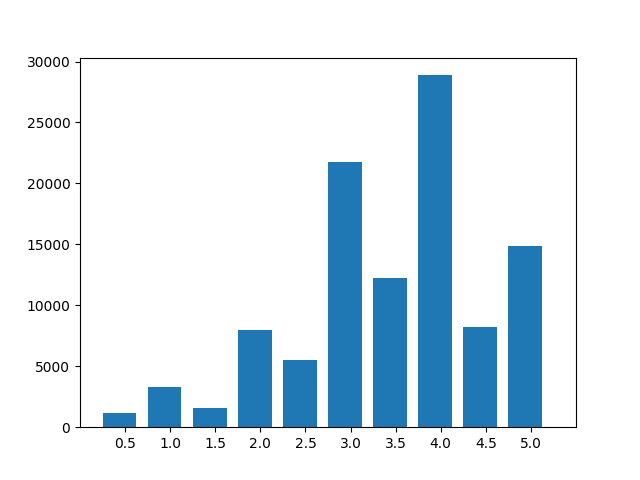
\includegraphics[scale=0.6]{small}
\caption{\emph{small} Movielens dataset ratings distribution}
\end{figure}

\begin{table}[H]
\centering
\begin{tabular}{l|r}
number of users N&  6040 \\ 
number of items M& 3706 \\
average rating & 3.58156 \\
standard deviation & 1.1171 \\
\end{tabular}
\caption{\emph{1M} Movielens dataset statistics}
\end{table}

\begin{figure}[H]
\centering
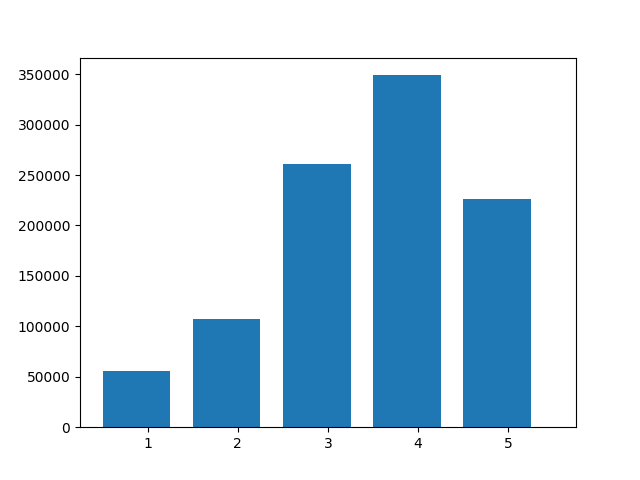
\includegraphics[scale=0.6]{1m}
\caption{\emph{1M} Movielens dataset ratings distribution}
\end{figure}


\section{Scaling issues and regularization}

In order to achieve the same intensity of learning per epoch even by varying
the minibatch size it is necessary to re-scale some hyperparameters.

Let's consider a complete objective for a typical learning task
of quantities $y_i$ from respective datapoints $x_i$, using
a dataset $\mathcal{D} = \{x_i,y_i\}_i^{|D|}$.
As the datapoints
are independent and identically-distributed, then it can be expressed as a sum over
all the datapoints.
One step of learning from this objective is usually referred as an "epoch".

\begin{nalign}
\label{complete_J}
J = \sum_{i=1}^{|\mathcal{D}|}
\ell(x_i,y_i) + \lambda \Omega(\Theta)
\end{nalign}

Where $\Omega$ is a regularization term, $\Theta$ is the set of the regularizable
parameters and $\lambda$ is a fixed hyperparamter that determines the regularization amount.

This objective is subject to Gradient Descent learning on the trainable parameters:

\begin{nalign}
\Theta_{t+1} = \Theta_t - \gamma\nabla_\Theta J_t
\end{nalign}

Where $\gamma$ is the learning rate hyperparameter.

As $J$ is defined as a sum over independent datapoints, it is possible to use Stochastic
Gradient Descent learning strategies, which take into account only a limited number of datapoints at each time.

It's desirable to consider the average contribution of each datapoint to the objective
$J$ \ref{complete_J}:

\begin{nalign}
\label{average_datapoint_J}
J_a = 
\frac{1}{|\mathcal{D}|}
J =
\frac{1}{|\mathcal{D}|}
\sum_{i=1}^{|\mathcal{D}|}
\ell(x_i,y_i) + \frac{\lambda}{|\mathcal{D}|} \Omega(\Theta)
\end{nalign}

If learning using $J_a$ is repeated $|\mathcal{D}|$ times within an epoch, then
the algorithm achieves the same learning intensity as
with $J$ by keeping the same learning rate $\gamma$.

By considering splitting the dataset and the objective $J$ 
\ref{complete_J} into a number of minibatches of size $B$, an approximation to $J_a$,
useful for SGD-like algorithms,
can be obtained:

\begin{nalign}
J_b = \frac{1}{B}\sum_{i=1}^{B} \ell (x_i, y_i) + \frac{\lambda}{|\mathcal{D}|}\Omega(\Theta)
\end{nalign}

An important consequence of using $J_b$ is that the intensity of the learning 
is altered,
because less updates would be applied to $\Theta$ at each epoch.
In order to balance this phenomenon, the learning rule can be modified as follows:

\begin{nalign}
\Theta_{t+1} = \Theta_t - B\gamma\nabla_\Theta J_{b,t}
\end{nalign}



\section{Prevention of exploding gradients}
It is possible, under specific circumstances, that the gradients may become unstable and
compromise the parameters of the model with infinities or "not a number" values.

In order to prevent this phenomenon, a few "tricks" have been implemented:

\paragraph{Gradient clipping}\cite{norm_clip} has been implemented with the
following norm-based scaling algorithm:

\begin{algorithm}
\caption{Norm-based gradient clipping}
\begin{algorithmic}[1]

\REQUIRE ~~\\
(1) Gradient tensor $\mathbf{g}$   \\
(2) Threshold $\theta$ (defaulted to value 10)
\ENSURE~~\\
(1) Scaled gradients $\hat{\mathbf{g}}$ whenever their L2 norm surpasses a threshold $\theta$.
`
\item[]
\IF{$||\mathbf{g}||_2 > \theta$}
    \STATE $\hat{\mathbf{g}} \leftarrow \frac{\theta}{||\mathbf{g}||_2}\mathbf{g}$
\ELSE
    \STATE $\hat{\mathbf{g}} \leftarrow \mathbf{g}$
\ENDIF
\RETURN $\hat{\mathbf{g}}$
\end{algorithmic}
\end{algorithm}

\paragraph{Scaled $\tanh$ activation function}. Some layers have 
"$\log\sigma$" outputs. As the output of these layers needs to be processed to
exponentiation in the likelihood function, if the activation is kept linear
there is a great risk of instability and value explosion.
For these reason a "pseudo-linear" soft-bounded activation function has been implemented
by re-scaling a $\tanh$ activation function.
A $\tanh$ activation function has the co-domain of the function bounded between -1 and +1.
Moreover, its derivative is approximately $1$ near the origin. It follows that $\tanh$
perfectly suits the role of pseudo-linear bounded activation function if it's rescaled as
follows:

\begin{nalign}
f(\mathbf{x}) = K * \tanh(\mathbf{x}/K)
\end{nalign}

Where $K$ is a small integer which is greater than 1. In this way this activation function
will be bounded between $-K$ and $+K$. A good value for $K$ might be 5, in order to obtain
$\sigma$-values properly bounded between $0.0067$ and $148.4$.

For layers that are supposedly linear in their outputs, such as Planar Flow's 
$\mathbf{w}$, $b$, and $\mathbf{u}$ quantities, as well as the means $\boldsymbol\mu$ of 
the gaussian distributions,
a "pseudo-linear" function
on the same guise has been implemented with $K=20$. 

\paragraph{Learning rate "warm-up"} has been implemented to prevent immediate divergence
in the first epochs due to steep gradients. 
Hence, the learning rate has been raised from a very small value
to regimen value during the course of the very first epochs.

\begin{algorithm}
\caption{Learning rate warm-up}
\begin{algorithmic}[1]

\REQUIRE ~~\\
(1) Initial learning rate $\gamma$   \\
(2) Current epoch number $t$ \\
(3) Number of initial warm-up epochs $K$ \\
(4) Base value of the warm up coefficient $B$  which has to be less than $1$
\ENSURE~~\\
(1) Adjusted and progressively increasing learning rate $\hat{\gamma}$ during the first $K$ epochs
\item[]
\IF{$t >= K$}
    \STATE $\hat{\gamma} = \gamma$
\ELSE
    \STATE $\hat{\gamma} = B^{K-t} \gamma$
\ENDIF
\RETURN $\hat{\gamma}$
\end{algorithmic}
\end{algorithm}

Appropriate parameter settings have been found as $K=3$ and $B=0.1$.


\section{Equivalences between AutoRec and VaeRec models}

In order to perform an adequate comparison between the AutoRec and VaeRec
models it's important to establish if there are any available equivalences.
In other words, it is interesting to see if a specific choice of hyperparameters
of the VaeRec leads to a model that is similar to the VaeRec both in its definition
and its performance.

Luckily such a model can be found in the VaeRec by setting the KL coefficient to 0.
This way that extra regularization term is absent and the VaeRec model becomes analogous
to the AutoRec model. An hypothesis can be formulated that in such similar models
the performances will be similar as well.

Experimental results confirm the hypothesis:

\begin{table}[H]
\centering
\begin{tabular}{c|c|c|c|r|r}
\thead{Minibatch \\size }& 
\thead{hid.layer \\ width }& 
\thead{num. hidden \\layers } &
\thead{latent z \\ dimensionality} & 
\thead{AutoRec (RProp) \\ testing RMSE }&
\thead{VaeRec (Adam) \\ testing RMSE }
\\
\hline
64 & 1000 & 1 & 250 & 
% harvest_autorec_20180625_122221 (adam)
0.8700
% harvest_autorec_20180723_114300 (pseudo_linear, and adam)
WAITING
& 
% harvest_vaerec_20180608_231009
0.8335
% harvest_vaerec_20180723_110214 (pseudo_linear)
WAITING
\\
64 & 1000 & 2 & 250 & 
% harvest_autorec_20180427_022040
0.8341 
% harvest_autorec_20180723_120629 (pseudo_linear, and adam)
WAITING
% harvest_autorec_20180723_122618/ (adam)
WAITING
& 
% harvest_vaerec_20180608_224259
0.8365 
% harvest_vaerec_20180723_115919 (pseudo_linear)
WAITING
\\
64 & 1000 & 1 & 500 & 
% NO (rprop)
% NO (adam)
% harvest_autorec_20180725_005108/ (pseudo_linear, and adam)
WAITING
& 
% NO (no gradient hacks)
% harvest_vaerec_20180725_004522/ (pseudo_linear)
WAITING
\\
64 & 1000 & 2 & 500 & 
% NO (rprop)
% NO (adam)
% harvest_autorec_20180725_005647/ (pseudo_linear, and adam)
WAITING
& 
% NO (no gradient hacks)
% harvest_vaerec_20180725_010335/ (pseudo_linear)
WAITING
\end{tabular}
\caption{Comparison of similar VaeRec and AutoRec models}
\end{table}

The testing error achieved by both AutoRec and VaeRec models
are very similar under similar hyperparameter settings.

\section{Progress curves}

Interesting information on how the model determines learning progress
can be obtained by observation of the RMSE progress over the epochs , both for the
training set and validation set. 
Analysis of these charts provides insight on issues such as choice of learning rate,
choice of learning rate annealing parameters, overfitting and underfitting.

\subsection{Tradeoff between KL divergence and weights regularization}

Both weights decay and KL divergence are regularizers that enable the model to achieve
generalization. The contribution of both these terms is compounded, so that 
coefficients need to be tuned in order to avoid over-regularization.

As an example, this can be seen in the following plot, where a VaeRec model
using L2 regularization with coefficient 200 is tested with, and without
the KL term:

% python3 plot_2.py harvest_vaerec_20180602_151546 harvest_vaerec_20180530_220845 "with kl" "without kl" --save text/with_kl_vs_without_kl.png
\begin{figure}[H]
\includegraphics[scale=0.7]{with_kl_vs_without_kl.png}
\caption{VaeRec with and without KL divergence, minibatch size set at 1}
\end{figure}

For additional comparison, here are the result by using a minibatch update schema
with size set at 64:

\begin{figure}[H]
\includegraphics[scale=0.7]{with_kl_vs_without_kl_mb64.png}
\caption{VaeRec with and without KL divergence, minibatch size set at 64}
\end{figure}

Using the minibatch shows considerable improvements for both variants (with and without KL
divergence).  It is interesting how the model with KL improves in such a drastic way
by using minibatch learning. This is probably caused by the KL regularizer being
very noisy with individual samples, causing over-regularization, as typical with SGD
(without minibatch) schemas. By using a minibatch
the KL regularizer becomes less noisy by smoothening via averaging. 


\chapter{Conclusion}

\begin{appendices}

\chapter{Derivations}
\section{Density of a transformed multivariate random variable}
\label{density_transformed}

a random variable $\mathbf{z}_0$ is transformed via an invertible transformation $\tr: \mathcal{R}^n \rightarrow \mathcal{R}^n$:
    
\begin{nalign}
\z{1} = \tr(\z{0})
\end{nalign}

Then, it's possible to express 
the pdf of $\z{1}$
by using the distribution of the original variable $\pz{0}{\z{0}}$ and
the invertible transformation $\tr$.

This can be demonstrated by making use of the cdf of $\z{1}$,
denominated $\Fz{1}{\z{1}}$, showing its relationship with the cdf of $\z{0}$
and the inverse of $\tr$\cite{transformed-density}:

\begin{nalign}
\Fz{1}{\gamma} &= \Pleq{\z{1}}{\gamma}\\
&= \Pleq{\tr(\z{0})}{\gamma} \\
&= \Pleq{\z{0}}{\trinv{\gamma}} \\
&= \Fz{0}{\trinv{\gamma}}
\end{nalign}

The integral is expanded and integration by substitution
is used to highlight the role of the pdf of $\z{0}$ and the determinant of
the Jacobian matrix of the inverse of $\tr$:
\begin{nalign}
\Fz{1}{\z{1}} 
&= \Fz{0}{\trinv{\z{1}}} \\
&=\int^{\trinv{\z{1}}} \pz{0}{\z{0}} \mathrm{d}{\z{0}}\\
&= \int^{\z{1}} \pz{0}{\trinv{\z{1}}} 
\cdot \abs{\det \Dtrinv{\z{1}} } \mathrm{d}{\z{1}}
\end{nalign}

Next, the derivative on $\z{1}$ is applied to the form of the 
cdf of $\z{1}$ just achieved, in order
to obtain a convenient formula for $\pz{1}{\z{1}}$:
\begin{nalign}
\pz{1}{\z{1}} 
&= \multipartial{1} \Fz{1}{\z{1}} \\
&= \multipartial{1}\int^{\z{1}} \pz{0}{\trinv{\z{1}}} 
\cdot \abs{\det \Dtrinv{\z{1}} } \mathrm{d}{\z{1}} \\
&= \pz{0}{\trinv{\z{1}}} \cdot \abs{\detDtrinv{\z{1}} }
\end{nalign}

The matrix inverse of the Jacobian matrix of an invertible function, such as $\tr$,
is the Jacobian matrix of $\tr^{-1}$: \cite{inverse-function-theorem}
    
\begin{nalign}
\left[\Dtr{\z{0}}\right]^{-1} &= \Dtrinv{\z{1}}
\end{nalign}

The well known property of the determinant of inverse matrix $\det(A^{-1})= 1/\det(A)$
can be used in order to just calculate the Jacobian of $\tr$ instead of the Jacobian of $\tr^{-1}$
. This leads to:

\begin{nalign}\label{trprob_with_detd}
\pz{1}{\z{1}} &= \pz{0}{\trinv{\z{1}}}\cdot \abs{\detDtr{\z{0}}}^{-1}
\end{nalign}

This form can be eventually be expressed as a function of $\z{0}$:

\begin{nalign}
\pz{1}{\z{1}} &= \pz{0}{\z{0}}\cdot \abs{\detDtr{\z{0}}}^{-1}
\end{nalign}

\section{Variational Expectation Lower Bound}

Given a 
dataset $\boldX = \{\boldxone \ldots \boldxN \}$
and the respective unobserved latent variable realizations
$\boldZ = \{\boldzone \ldots \boldzN\}$
\cite{Fox2012}
suggest to derive a quantity to be maximized by considering the minimization
of the Kullback-Leibler divergence $\kl{\qphiZ}{\pZcond}$ by decomposing it as follows:

\begin{nalign}
\kl{\qphiZ}{\pZcond} &=
\expectqphiZ{\log \frac{\qphiZ}{\pZcond}}\\
&= \expectqphiZ{\log \qphiZ - \log \pXcond - \log \pZ + \log \pX}
\end{nalign}

As the integrand inside the expectation $\expectqphiZ{\log \pX}$ 
is a constant w.r.t. $\boldZ$, then $\expectqphiZ{\log \pX}=\log \pX$. Hence, the
previous expression can be rewritten as:

\begin{nalign}
\log \pX &= \kl{\qphiZ}{\pXcond}
+ \elboX
\end{nalign}

Where we made use of this shorthand:
\begin{nalign}
    \elboX = \expectqphiZ{-\log \qphiZ + \log \pXcond + \log \pZ}
\end{nalign}

As $\log \pX$ is a constant w.r.t. the variational parameters $\phi$,
and $\kl{\qphiZ}{\pXcond}$ is always non-negative,
then the quantity $\elboX$ can be interpreted as a lower-bound to $\log \pX$
whose maximization implies the minimization of $\kl{\qphiZ}{\pXcond}$.

The lower-bound $\elboX$ can also be expressed, as in \cite{1312.6114},
by grouping some terms
into a negative Kullback-Leibler divergence:
\begin{nalign}
\elboX 
&= -\kl{\qphiZ}{\pZ} + \expectqphiZ{\log \pXcond}
\end{nalign}

The Kullback-Leibler divergence $\kl{\qphiZ}{\pZ}$ can be also expressed by 
an entropy and a cross-entropy term, hence:

\begin{nalign}\label{elbo_crossentropy}
\elboX 
&= -\entropy{\qphiZ,\pZ} + \entropy{\qphiZ} + \expectqphiZ{\log \pXcond}
\end{nalign}

More commonly, the lower-bound is re-arranged by making use of
the entropy of the variational approximation
and expectation over the joint probability:

\begin{nalign}
\elboX = \entropy{\qphiZ} + \expectqphiZ{\log \pXZ}
\end{nalign}




\section{ELBO as sum of terms dependent on individual datapoints}
\label{elbo_datapoint}

As used by \cite{1312.6114}, the ELBO can be decomposed into
a sum of terms, each dependent only on an individual datapoint. 
This follows the assumption that each datapoint generated by a certain
latent variable realization is independent from both the other datapoints:
\begin{nalign}
\pXcond = \prod_{i=1}^N \pxicondi
\end{nalign}

Same assumption is made on the prior distribution on the latent variables:
\begin{nalign}
\pZ = \prod_{i=1}^N \pzi
\end{nalign}

Hence this is the form for the joint probability:
\begin{nalign}
\pXZ = \pXcond \pZ &= \prod_{i=1}^N \pxicondi \pzi = \prod_{i=1}^N \pxizi
\end{nalign}

For convenience, the chosen form for $\elboX$
will be the \eqref{elbo_crossentropy}.

It's possible to make use of information-theoretical properties
\cite{Bergstrom2008}:

\begin{nalign}
\entropy{\qphiZ} &= \entropy{\qphizone} &&\\
    &+ \entropy{\qphiZminusone | \qphizone} 
 && \text{chain rule for joint entropy}\\
 &= \entropy{\qphizone} + \entropy{\qphiZminusone}
 && \text{independence of datapoints}\\
 &= \sum_i \entropy{\qphizi }
 && \text{recursion}
\end{nalign}

Similarly, for $\entropy{\qphiZ,\pZ}$:

\begin{nalign}
\entropy{\qphiZ,\pZ} &= \entropy{\qphizone,\pzone} 
+ \entropy{\qphiZminusone, \pZminusone | \qphizone, \pzone} 
\\
 &= \entropy{\qphizone,\pzone} + \entropy{\qphiZminusone,\pZminusone}
\\
&= \sum_i \entropy{\qphizi,\pzi} 
\end{nalign}

For the third term $\expectqphiZ{\log \pXcond}$:
\begin{nalign}
\expectqphiZ{\log \pXcond} &= \integral{\boldzone}{\cdots \integral{\boldzN}{
    \prod \qphizi \sumiN \log \pxicondi
}\cdots} \\
&= \integral{\boldzone}{\qphizone \cdots \integral{\boldzN}{
     \qphizN \sumiN \log \pxicondi
}\cdots} \\
&= \sumiN \integral{\boldzi}{\qphizi \log \pxicondi}\\
&= \sumiN \expectqphizi{\log \pxicondi}
\end{nalign}

By plugging these forms into the ELBO \eqref{elbo_crossentropy},
it can be shown as a sum of individual objective terms, each of those
is dependent on only a single datapoint:
\begin{nalign}
\elboX = \sumiN -\entropy{\qphizi,\pzi} + \entropy{\qphizi } + \expectqphizi{\log \pxicondi}
\end{nalign}

It's noteworthy that $\elboX$ can be expressed by the following mutual information term: 

\begin{nalign}
    \mutinf{\boldz}{\boldx} &= \expectx{\kl{\qphiz}{\pzonly}}\\
        & \approx \frac{1}{N}\sumiN \kl{\qphizi}{\pzi}
\end{nalign}

Hence the $\elboX$ can be expressed as:

\begin{nalign}
\elboX = - N\cdot \mutinf{\boldz}{\boldx} + \sumiN \expectqphizi{\log \pxicondi}
\end{nalign}

\section{Rearranging the variational lower bound}

The term $\kl{\qphizcondi}{\pthetaz}$ has an analytical solution within the original
VAE framework with Gaussian approximation of the posterior, 
whence it's not subject to Monte-Carlo sampling.

Unfortunately, by using Normalizing Flows, the $\mathbb{KL}$ cannot be determined
analytically, so it has to be subject to Monte-Carlo sampling.
The negative lower bound $\mathcal{L}(x)$ can be interpreted as
a negative Free-energy (FIXME: look what is "free energy) $-\mathcal{F}(x)$
that has to be minimized.

It's useful to reduce the free energy into it's "atomic" probability components:

\begin{nalign}
\freeenergyxi &= -\elboxi\\
    &= -\expectqphi{\logpjointi - \logqzcondi} \\
    &= \expectqphi{-\logpxicond - \logpz + \logqzcondi}
\end{nalign}

The random multivariate variable $\boldz$ can be interpreted as being the result
of a transformation $\boldz = \tr(\boldzzero)$ of an initial random multivariate variable 
which happens to have a simple distribution, such as multivariate gaussian 
with diagonal covariance matrix.

For the \emph{law of the unconscious statistician} (LOTUS) \cite{lotus} (FIXME: expand)
the energy can have a form with expectations over the simpler distribution of
$\boldzzero$:

\begin{nalign}
\freeenergyxi &= \expectqzero{- \logpxicondtr - \logptr}
+ \expectqphi{\logqzcondi}
\end{nalign}

The last term is clearly the negative entropy of $\qzcondi$:
\begin{nalign}
 \entropyqzcondi &= - \expectqphi{\logqzcondi}
\end{nalign}
    
At this point the previous result on the transformed density can be used in order to express this term as a function of $\qzero$:

\begin{nalign}
    \logqzcondi &= \log q_0(\trinv{\boldz}) + \log \left( |\detDtr{\boldz}|^{-1} \right)\\
     &= \log q_0(\trinv{\boldz}) - \log \left( |\detDtr{\boldz}| \right)
\end{nalign}

By applying the \emph{law of the unconscious statistician} to $-\entropyqzcondi$,
a relationship between the entropy of the two distributions emerges:

\begin{nalign}
     -\entropyqzcondi &= \expectqphi{\logqzcondi}\\
    &= \expectqphi{\log q_0(\trinv{\boldz}) - \log \left( |\detDtr{\boldz}| \right)}\\
    &= \expectqzero{\log q_0(\trinv{\tr(\boldzzero)})}
       - \expectqzero{\log \left( |\detDtr{\tr(\boldzzero)}| \right)}\\
    &= \expectqzero{\log q_0(\boldzzero)}
       - \expectqzero{\log \left( |\detDtr{\tr(\boldzzero)}| \right)}\\
    &= - \entropyqzero - \expectqzero{\log \left( |\detDtr{\tr(\boldzzero)}| \right)}
\end{nalign}


\subsection{A closer look to the terms of the free energy}


Finally, it's possible to write $\freeenergyxi$ in the following form:
\begin{align}
\freeenergyxi = &- \expectqzero{\logpxicondtr} \\
    &- \expectqzero{\logptr} \\
    &- \entropyqzero \\
    &- \expectqzero{\log \left( |\detDtr{\tr(\boldzzero)}| \right)}
\end{align}



\section{Jacobian of a Planar Transformation}
\label{jacobian_illt}

The Jacobian $\partialboldz{t(\boldz)}$ of the transformation can be found as follows:

\begin{nalign}
\partialboldz{\boldz} &= \identity \\
\partialboldz{\wt \boldz + b} &= \wt && \text{The Jacobian of a scalar is a row vector} \\
\partialboldz{h(\wt \boldz + b)} &= h^\prime (\wt \boldz + b)\wt && \text{Chain rule}
\end{nalign}

Hence:
\begin{nalign}
\partialboldz{t(\boldz)} &= \identity + \boldu h^\prime(\wt \boldz + b)\wt
\end{nalign}

In order to derive the determinant of the Jacobian, it's possible to make use of the
\emph{matrix determinant lemma} which states:
\begin{nalign}
    \det ( \boldA + \bolda \boldbt ) = (1 + \boldbt \boldAinv \bolda)(\det \boldA)
\end{nalign}

Considering $\boldA = \identity$, $\bolda = \boldu$ and $\boldbt = h^\prime(\wt \boldz + b)\wt$,
this leads to:

\begin{nalign} \label{detjacobian_iltt}
\det \partialboldz{t(\boldz)} &= \det(\identity + \boldu h^\prime(\wt \boldz + b) \wt)\\ 
&= (1 + h^\prime(\wt \boldz + b)\wt \identity^{-1} \boldu)(\det \identity)\\
 &=1 + h^\prime(\wt \boldz + b)\wt \boldu
\end{nalign}


\section{Energy of single invertible linear-time transformation step}\label{energy_of_1step_illt}

\subsection{Model form}
As a simple case let's derive the free-energy objective function by using the
following model: 
\paragraph{The transformation $\tr$} is made of a single invertible linear-time transformation step.
\paragraph{The distribution $\qzero$ of the initial sample $\boldzzero$} is assumed
to be a simple
Multivariate Normal with diagonal covariance matrix.
\paragraph{The likelihood distribution $\pxicondtr$} is also assumed to be  
a Multivariate Normal with diagonal covariance matrix.
\paragraph{Prior distribution on the transformed latent code} 
is a spherical Multivariate Normal with Identity covariance matrix centered on 0.

\subsection{Derivation of the free-energy $\freeenergyxi$}
Follows the derivation of a Monte Carlo 1-sample approximation of $\freeenergyxi$:
\paragraph{The likelihood term}
\begin{nalign}
\expectqzero{\logpxicondtr} 
&\approx - \log\left(\sqrt{2\pi\abs{\Sigma_\theta}}\right)
-\half \transpose{\diffximutheta} \Sigma^{-1}_\theta \diffximutheta \\
&= -\half \log\left( 2\pi \right)
-\half \sum_j \log \sigma_{\theta j}
-\half \sum_j 
        \diffxijmuthetaj^2 \cdot \frac{1}{\sigma_{\theta j}}
\end{nalign}
It can be seen how this term expresses a regression error.

\paragraph{The prior term on the transformed latent code.}
The derivation for this term is made easy by the 
parameters of the prior 
($\boldsymbol\mu = \mathbf{0}$,$\boldsymbol\Sigma = \identity$).
\begin{nalign}
\expectqzero{\logptr} 
&\approx - \log\left(\sqrt{2\pi\abs{\identity}}\right)
-\half \transpose{\diffTxizerotheta} \identity^{-1} \diffTxizerotheta \\
&= -\half \log\left( 2\pi \right)
-\half \ltwonorm{\tr(\boldzzero)}
\end{nalign}
The form of this term highlight its function as a regularizer.

\paragraph{The entropy term on the initial code.}
The entropy of a Multivariate Normal distribution is: $\half \log\left((2\pi)^k\abs{\boldsymbol\Sigma}\right)$, hence the entropy of the initial sample $\boldzzero$ can be derived as:

\begin{nalign}
\entropyqzero &\approx \half \log\left(2\pi\right) + \half k + \half \sum_j\log \sigma_{\phi j}
\end{nalign}

\paragraph{The transformation term}
Follows the derivation 
\eqref{detjacobian_iltt}:
\begin{nalign}
\expectqzero{\log \left( \abs{\detDtr{\boldzzero}} \right)} 
&\approx \log \abs{ 1 + h^\prime(\wt \boldzzero + b)\wt \boldu }
\end{nalign}

\subsubsection{Free-energy $\freeenergyxi$ implementation with the Invertible Linear-time Transformation }

By summing all the terms and removing the constant terms,
this is the form of approximation of the free-energy $\freeenergyxi$ objective:

\begin{nalign}
\freeenergyxi
\approx &
\half \sum_j \log \sigma_{\theta j}\\
&+\half \sum_j \left[
        \diffximutheta_{[j]}
    \right]^2 \cdot \frac{1}{\sigma_{\theta j}}\\
&+ \half \ltwonorm{\tr(\boldzzero)}\\
&-\half \sum_j\log \sigma_{\phi j}\\
&- \log \abs{ 1 + h^\prime(\wt \boldzzero + b)\wt \boldu }\\
\end{nalign}

\section{Multiple nested transformation steps}\label{multiple_iltt_steps}

\begin{figure}
\caption{Average squared error of a VAE with Normalizing Flows trained
         on the MNIST dataset. Parameters are: learning rate $5*10^{-7}$,
         activation functon sigmoid, latent dimensionality 16,
         size of the hidden layer 64. The three experiments are differentiated
         by the NF's K being 4, 5 and 6. The plot demonstrates that,
         as K gets larger, the reconstruction error deminishes over the 1300 epochs.
         The optimizer used is Adam.}
\centering
\includegraphics[width=13cm]{mnist_nfk456.eps}
\end{figure}

A transformation $\tr(\boldz)$ might be composed
of multiple nested but similar transformation steps
each with it's own parameters:

\begin{nalign}
\tr(\boldz) &= t_k \circ t_{k-1} \circ \ldots \circ t_1(\boldzzero)
\end{nalign}

By using the chain rule, the gradient of the transformation becomes:
\begin{nalign}
\Dtr{\boldzzero}
&= \prodk{\derivtk{\boldzkminusone}}
\end{nalign}

The determinant of the product of square matrices is the product of their determinants, hence:
\begin{nalign}
\det \Dtr{\boldzzero} &= \prodk{\det \derivtk{\boldzkminusone}}
\end{nalign}

The expectation term, as previously illustrated, can be approximated with
a single Monte Carlo sample:

\begin{nalign}
\expectqzero{\log \left( \abs{\Dtr{\boldzkminusone}} \right)}
&\approx \log \abs{\prodk{\det \derivtk{\boldzkminusone}}}
\\
&=\sumk{ \log \abs{\derivtk{\boldzkminusone}}}
\end{nalign}
\subsection{Implementation with Invertible Linear-time Transformations}

With invertible Linear-time Transformations, the derivative becomes:

\begin{nalign}
\Dtr{\boldzzero}
&=\prodk{ \identity + \bolduk h^\prime(\wtk \boldzkminusone + \bk)\wtk }
\end{nalign}

The expectation sample becomes:

\begin{nalign}
\expectqzero{\log \left( \abs{\Dtr{\boldzkminusone}} \right)}
&\approx
\sumk{ \log \abs{1 + h^\prime(\wtk \boldzkminusone + \bk)\wtk \bolduk }}
\end{nalign}


\section{Derivation of Kullback-Leibler divergence between diagonal-covariance Gaussian posterior approximation and spherical Gaussian prior}

The Variational-Autoencoder introduced by \cite{1312.6114} makes use of a posterior approximation that takes the form of a diagonal-covariance Normal distribution
$\qzcond = \normal{\boldz}{\boldmu}{\boldsigma}$;
the prior distribution on the latent codes has a spherical Gaussian distribution with $\Sigma = I$ and $\boldmu = \boldzero$. Dimensionality of $\boldz$ is $J$.
Follows a derivation which ends up in a convenient form:

\begin{nalign}
\kl{\qzcond}{\pzonly} &= \integral{\boldz}{\qzcond \left(\logqzcond - \logpz \right)}
\end{nalign}

By considering separately the two terms one obtains:

\begin{nalign}
\integral{\boldz}{\pzonly \logpz} &= \integral{\boldz}{\pzonly \left[\log \left( \left((2\pi)^J |\mathbf{I}| \right)^{-\half}\right)- \half (\transpose{\boldz} \mathbf{I}^{-1}\boldz )\right]} \\
    &= -\half\left[J \log{2\pi} + \expectqph{\transpose{\boldz}\boldz}\right] \\
    &= -\half\left[J \log{2\pi} + \left( \trace{\boldSigma} + \transpose{\boldmu}\boldmu \right)\right] \\
    &= -\half\left[J \log{2\pi} + \left( \sumj{\sigma_j^2} + \sumj{\mu_j^2} \right) \right]\\
\end{nalign}

Where the trick $\expect{\boldx}{\transpose{\boldx}\mathbf{A}\boldx} = \trace{\mathbf{A}\boldSigma} + \transpose{\mathbf{m}}\mathbf{A}\mathbf{m}$ from \cite{cookbook} has been used.

Second term is:
\begin{nalign}
\integral{\boldz}{\pzonly \logpz} &= -\half\left[ J\log (2\pi) + \log (|\boldSigma| ) + \expectqph{\transpose{(\boldz - \boldmu)} \boldSigma^{-1}(\boldz - \boldmu)} \right]\\
    &= -\half\left[ J\log (2\pi) + \log (|\boldSigma| ) +\transpose{(\boldmu - \boldmu)} \boldSigma^{-1}(\boldmu - \boldmu) + \trace{\boldSigma^{-1}\boldSigma}\right]\\
    &= -\half\left[ J\log (2\pi) + \sumj{\log \sigma_j^2} + J \right]\\
\end{nalign}

Where the trick  $\expect{\boldx}{\transpose{(\boldx - \mathbf{m^\prime})}\mathbf{A}(\boldx - \mathbf{m^\prime})} = \trace{\mathbf{A}\boldSigma} + \transpose{(\mathbf{m} - \mathbf{m^\prime})}\mathbf{A}(\mathbf{m} - \mathbf{m^\prime})$ from \cite{cookbook} has been used.

Putting the two terms together:

\begin{nalign}\label{kl_multivariate}
\kl{\qzcond}{\pzonly} &= \half \left[ \sumj{\sigma_j^2} + \sumj{\mu_j^2} - \sumj{\log \sigma_j^2} - J \right]\\
    &= \half \sumj{ \sigma_j^2 + \mu_j^2 - \log \sigma_j^2 - 1}
\end{nalign}

\subsection{KL of diagonal covariance gaussians is a sum of the KL of the individual variables}

A Gaussian pdf with diagonal covariance matrix can be decomposed into a product of the
individual independent latent variables. 

First, the diagonal-covariance Gaussian can be interpreted as the product of
individual one-dimensional independent Gaussian variables:

\begin{nalign}
\normal{\boldx}{\boldmu}{\boldSigma} &= \left((2\pi)^J |\boldSigma|\right)^{-\half}
\exp\left\{-\half \transpose{(\boldx - \boldmu)}\boldSigma^{-1}(\boldx - \boldmu)\right\} \\
 &= \left[\prodj{(2\pi\sigma_j^2)^{-\half}}\right]\exp\left\{-\half\left[\sumj{\transpose{(x_j-\mu_j)}\frac{1}{\sigma_j^2}(x_j-\mu_j)\right]}\right\} \\
 &= \left[\prodj{(2\pi\sigma_j^2)^{-\half}}\right]\exp\left\{-\half\transpose{(x_j-\mu_j)}\frac{1}{\sigma_j^2}(x_j-\mu_j)\right\}\\
 &= \prodj{\normal{x_j}{\mu_j}{\sigma^2_j}}
\end{nalign}

This fact can be used to get to a simpler way to calculate the KL divergence:
\begin{nalign}\label{kl_as_sum}
\kl{\qzcond}{\pzonly} &= \integral{\boldz}{\left[\prodjprime{q(z_{j^\prime}|\boldx)}\right] \left\{ \log\left[\prodj{q(z_j|\boldx)}\right] - \log\left[\prodj{p(z_j)}\right]\right\}}\\
 &= \integral{\boldz}{\left[\prodjprime{q(z_{j^\prime}|\boldx)}\right]\exp\left\{\sumj{\log q(z_j|\boldx) - \log p(z_i)}\right\}}\\
 &= \sumj{\integral{\boldz}{\left[\prodjprime{q(z_{j^\prime}|\boldx)}\right]\exp\left\{\log q(z_j|\boldx) - \log p(z_i)\right\}}}\\
 &= \sumj{\integral{z_j}{\left[\log q(z_j|\boldx) - \log p(z_j)\right]q(z_j|\boldx)}}\underbrace{\integral{\boldz_{-j}}{q(\boldz_{-j}|\boldx)}}_{=1} \\
 &= \sumj{\kl{q(z_j|\boldx)}{p(z_j)}}
\end{nalign}

Where $\boldz_{-j}$ are the latent variables excluding $z_j$.

\subsection{KL of a one-dimensional Gaussian vs unit circle (FIXME: name??) Gaussian}

The Kullback-Leibler divergence of an arbitrary one-dimensional Gaussian $q(z) = \normal{z}{\mu}{\sigma^2}$
versus
a unit circle Gaussian $p(z)=\normal{z}{0}{1}$ can be derived as follows:

\begin{nalign}\label{kl_one_d}
\kl{q(z)}{p(z)} &= \expect{q}{\log q(z) - \log p(z)} \\
&= \half \left[ -\log(2\pi\sigma^2) - \frac{1}{\sigma^2}\expect{q}{z^2} + \frac{2\mu}{\sigma^2} \expect{q}{z} - \frac{\mu^2}{\sigma^2} + \log{2\pi} + \expect{q}{z^2} \right]\\
&= \half \left[ - \log(2\pi\sigma^2) - \frac{1}{\sigma^2}(\mu^2 + \sigma^2) + \frac{2\mu^2}{\sigma^2} - \frac{\mu^2}{\sigma^2} + \log{2\pi} + \mu^2 + \sigma^2 \right]\\
&= \half \left[ - \log\sigma^2 - 1 + \mu^2 + \sigma^2 \right]
\end{nalign}

This allows us to get the same result as $\ref{kl_multivariate}$ by easily combining \ref{kl_as_sum} with \ref{kl_one_d}.

\end{appendices}


%\section{Baseline model}

The baseline model that has been employed was the \emph{PMF1} model as described in the original Probabilistic Matrix Factorization paper.

The parameters for the two Gaussian priors have been set to $100$ for $\sigma_U$ and $1000$ for $\sigma_V$. The $\sigma_R$ scale parameter for the ratings has been set at $1$.
This is in compliance with the corresponding regularization parameters $\lambda_U=0.01$ and $\lambda_V=0.001$ of the \emph{PMF1} model.

Instead of using SGD with momentum as the original paper proposed, Adam gradient descent was herein been employed, with parameters $\beta_1=0.9$, $\beta_2=0.999$ and $\epsilon=10^{-8}$. The gradients have been jointly calculated for every rating in the training set and also jointly applied to the latent vectors $U_i$ and $V_j$ at every step.

The epochs have been implemented with a schema that made possible to achieve a level of randomization and at the same time efficiency in retrieving data from disk.

The learning rate has been also set to $0.005$ as in \emph{PMF1}.
% NOT TRUE:, but with a slowly decaying rate over the 2000 epochs. At the end of each training experiment the learning rate would be halved to $0.0025$, as the annealing parameter $T$ has been set equal to the number of epochs, 2000.

These differences in experimental settings made it possible for the 
\emph{PMF1} model to achieve an even lower testing RMSE than the one that was reported, down to FIXME, instead of the previously reported 0.9430.

The validation set has been chosen as the first chunk of the randomized dataset, hence consisting in $2^17 = 131072$ ratings.

\subsection{Dataset random permutation schema}
As a preliminary measure to avoid correlations between ratings in the same chunks, the 
dataset had its rows shuffled before the experiments were run.
The dataset has been divided in chunks, each of size $2^{16}=65336$ ratings.
Each epoch processed every chunk. This means that every datapoint in the dataset was processed 
exactly one time. This is important to ensure that each rating has the same influence
in the learning process.
Within one epoch, the order of the chunks was randomly permuted. 
Each chunk was then read into memory following this random permutation order and processed. 
After a chunk is processed, the memory allocated by it is freed and the following 
chunk in the random permutation order is loaded. 
Moreover, the order of datapoints processing has been randomized within each individual chunk.
This has been implemented without actually shuffling the datapoints in memory, but just
by accessing them using a permutation of their indexes.

\begin{algorithm}
\caption{Memory and disk-read efficient dataset randomization schema for SGD-like updates}
\label{code:1}
\begin{algorithmic}[1]

\REQUIRE ~~\\
(1) Dataset $\mathcal{D}$\\
(2) $\mathrm{\#epochs}$\\
(3) $\chunklen$\\
(4) Model parameters $\theta$\\
(5) Latent variables $\Z$
\ENSURE~~\\
(1) Inference and learning using each datapoint in the dataset once for every epoch\\
(2) High degree of randomization the order of the datapoints\\
(3) Few disk and memory operations

\item[]
\STATE Let $\dataset \leftarrow \mathtt{shuffle}(\dataset)$
\STATE Let $\nchunks \leftarrow \mathtt{ceiling}(|\dataset|/\chunklen)$
\FOR{ $e$ in $(1\ldots \mathtt{\#epochs})$}
\FOR{ $i$ in $\randperm{1\ldots \nchunks}$} 
\STATE Let $\chunk \leftarrow \mathtt{read\_chunk}\left(i\right)$
\FOR{ $j$ in $\randperm{1\ldots |\chunk|}$}
\STATE Let $\datapoint \leftarrow \chunk[j]$
\STATE Let $\theta,\Z \leftarrow \mathtt{update}(\datapoint,\theta,\Z)$
\ENDFOR
\ENDFOR
\ENDFOR
\end{algorithmic}
\end{algorithm}


%\section{Model with separated neural networks that produce vectors joined by dot product}

As a first experiment with models more complex than simple PMF, a single-layer neural model with two separated 
neural networks fed respectively by user and item vectors has been employed.
The two neural networks produce deterministically two vectors of the same size of the latent vectors. Those output vectors are joined by a dot product and a final logistic function in order to provide a rating prediction, exactly like the original PMF models.

The likelihood of a rating, given the model can be formalized as follows:

\begin{equation}
p(R_{ij}|u_i,v_j) = \mathcal{N}(R_{ij}|g(\net{u}{u_i}\cdot\net{v}{v_j}),\sigma)
\end{equation}

Each network has this simple structure:
\begin{equation}
\net{}{\mathbf{z}} = g(\mathbf{z} \cdot W + \mathbf{b})
\end{equation}

$g$ is defined as the logistic function $g(\mathbf{t}) = \frac{1}{1 + e^{-\mathbf{t}}}$

\subsection{Experiments}

Experiment settings have been kept identical to the evaluation of the baseline PMF model.

This model exhibits a very fast learning in the early epochs, which is measured by a quick drop in validation error much faster than PMF, unfortunately followed by a plateau at FIXMEINSERTVALUEHERE as can be seen from this plot:

    FIXME INSERT PLOT

\subsection{Discussion}

Alternating learning of parameters of the neural network and latent vectors
with gradient descent has been proposed by FIXMECITEALTERNATINGPAPER,
technique that they called Alternating Back-Propagation (ABP).

This raises some concerns, as the neural network, at the beginning,
is going to be trained to reduce the error
on the basis of randomly
initialized vectors.
Likewise, the latent vectors are going to be optimized on the basis of a randomly-initialized neural network.

This problem is already posed in other unsupervised learning techniques, such as the EM algorithm. One of the main differences from EM is that for each updating step, E or M, the optimum
solution is found, while ABP uses gradient descent to progressively find an optimimum.
This allows freedom to choose how much influential each of the two steps (updating parameters
or latent variables) can be. The choice can be expressed by leaving more iterations to update
the parameters or to the latent variables, as well as choosing different learning rates for the two steps.

An better idea for an alternation could be make ABP behave more like EM.
Considering a single step of updating latent variables or parameters,
this step might be left only once there is quite some confidence
that the quantity to be optimized
has reached an optimum.
This optimum is possibly reached once the magnitude of the gradients has become much
lower than at the beginning of the step. Once this condition has been assessed,
it's possible to end the updating step and switching to the other quantity, as in EM.




%\section{Density of a transformed multivariate random variable}
\label{density_transformed}

a random variable $\mathbf{z}_0$ is transformed via an invertible transformation $\tr: \mathcal{R}^n \rightarrow \mathcal{R}^n$:
    
\begin{nalign}
\z{1} = \tr(\z{0})
\end{nalign}

Then, it's possible to express 
the pdf of $\z{1}$
by using the distribution of the original variable $\pz{0}{\z{0}}$ and
the invertible transformation $\tr$.

This can be demonstrated by making use of the cdf of $\z{1}$,
denominated $\Fz{1}{\z{1}}$, showing its relationship with the cdf of $\z{0}$
and the inverse of $\tr$\cite{transformed-density}:

\begin{nalign}
\Fz{1}{\gamma} &= \Pleq{\z{1}}{\gamma}\\
&= \Pleq{\tr(\z{0})}{\gamma} \\
&= \Pleq{\z{0}}{\trinv{\gamma}} \\
&= \Fz{0}{\trinv{\gamma}}
\end{nalign}

The integral is expanded and integration by substitution
is used to highlight the role of the pdf of $\z{0}$ and the determinant of
the Jacobian matrix of the inverse of $\tr$:
\begin{nalign}
\Fz{1}{\z{1}} 
&= \Fz{0}{\trinv{\z{1}}} \\
&=\int^{\trinv{\z{1}}} \pz{0}{\z{0}} \mathrm{d}{\z{0}}\\
&= \int^{\z{1}} \pz{0}{\trinv{\z{1}}} 
\cdot \abs{\det \Dtrinv{\z{1}} } \mathrm{d}{\z{1}}
\end{nalign}

Next, the derivative on $\z{1}$ is applied to the form of the 
cdf of $\z{1}$ just achieved, in order
to obtain a convenient formula for $\pz{1}{\z{1}}$:
\begin{nalign}
\pz{1}{\z{1}} 
&= \multipartial{1} \Fz{1}{\z{1}} \\
&= \multipartial{1}\int^{\z{1}} \pz{0}{\trinv{\z{1}}} 
\cdot \abs{\det \Dtrinv{\z{1}} } \mathrm{d}{\z{1}} \\
&= \pz{0}{\trinv{\z{1}}} \cdot \abs{\detDtrinv{\z{1}} }
\end{nalign}

The matrix inverse of the Jacobian matrix of an invertible function, such as $\tr$,
is the Jacobian matrix of $\tr^{-1}$: \cite{inverse-function-theorem}
    
\begin{nalign}
\left[\Dtr{\z{0}}\right]^{-1} &= \Dtrinv{\z{1}}
\end{nalign}

The well known property of the determinant of inverse matrix $\det(A^{-1})= 1/\det(A)$
can be used in order to just calculate the Jacobian of $\tr$ instead of the Jacobian of $\tr^{-1}$
. This leads to:

\begin{nalign}\label{trprob_with_detd}
\pz{1}{\z{1}} &= \pz{0}{\trinv{\z{1}}}\cdot \abs{\detDtr{\z{0}}}^{-1}
\end{nalign}

This form can be eventually be expressed as a function of $\z{0}$:

\begin{nalign}
\pz{1}{\z{1}} &= \pz{0}{\z{0}}\cdot \abs{\detDtr{\z{0}}}^{-1}
\end{nalign}

%\section{Variational Expectation Lower Bound}

Given a 
dataset $\boldX = \{\boldxone \ldots \boldxN \}$
and the respective unobserved latent variable realizations
$\boldZ = \{\boldzone \ldots \boldzN\}$
\cite{Fox2012}
suggest to derive a quantity to be maximized by considering the minimization
of the Kullback-Leibler divergence $\kl{\qphiZ}{\pZcond}$ by decomposing it as follows:

\begin{nalign}
\kl{\qphiZ}{\pZcond} &=
\expectqphiZ{\log \frac{\qphiZ}{\pZcond}}\\
&= \expectqphiZ{\log \qphiZ - \log \pXcond - \log \pZ + \log \pX}
\end{nalign}

As the integrand inside the expectation $\expectqphiZ{\log \pX}$ 
is a constant w.r.t. $\boldZ$, then $\expectqphiZ{\log \pX}=\log \pX$. Hence, the
previous expression can be rewritten as:

\begin{nalign}
\log \pX &= \kl{\qphiZ}{\pXcond}
+ \elboX
\end{nalign}

Where we made use of this shorthand:
\begin{nalign}
    \elboX = \expectqphiZ{-\log \qphiZ + \log \pXcond + \log \pZ}
\end{nalign}

As $\log \pX$ is a constant w.r.t. the variational parameters $\phi$,
and $\kl{\qphiZ}{\pXcond}$ is always non-negative,
then the quantity $\elboX$ can be interpreted as a lower-bound to $\log \pX$
whose maximization implies the minimization of $\kl{\qphiZ}{\pXcond}$.

The lower-bound $\elboX$ can also be expressed, as in \cite{1312.6114},
by grouping some terms
into a negative Kullback-Leibler divergence:
\begin{nalign}
\elboX 
&= -\kl{\qphiZ}{\pZ} + \expectqphiZ{\log \pXcond}
\end{nalign}

The Kullback-Leibler divergence $\kl{\qphiZ}{\pZ}$ can be also expressed by 
an entropy and a cross-entropy term, hence:

\begin{nalign}\label{elbo_crossentropy}
\elboX 
&= -\entropy{\qphiZ,\pZ} + \entropy{\qphiZ} + \expectqphiZ{\log \pXcond}
\end{nalign}

More commonly, the lower-bound is re-arranged by making use of
the entropy of the variational approximation
and expectation over the joint probability:

\begin{nalign}
\elboX = \entropy{\qphiZ} + \expectqphiZ{\log \pXZ}
\end{nalign}




%\section{ELBO as sum of terms dependent on individual datapoints}
\label{elbo_datapoint}

As used by \cite{1312.6114}, the ELBO can be decomposed into
a sum of terms, each dependent only on an individual datapoint. 
This follows the assumption that each datapoint generated by a certain
latent variable realization is independent from both the other datapoints:
\begin{nalign}
\pXcond = \prod_{i=1}^N \pxicondi
\end{nalign}

Same assumption is made on the prior distribution on the latent variables:
\begin{nalign}
\pZ = \prod_{i=1}^N \pzi
\end{nalign}

Hence this is the form for the joint probability:
\begin{nalign}
\pXZ = \pXcond \pZ &= \prod_{i=1}^N \pxicondi \pzi = \prod_{i=1}^N \pxizi
\end{nalign}

For convenience, the chosen form for $\elboX$
will be the \eqref{elbo_crossentropy}.

It's possible to make use of information-theoretical properties
\cite{Bergstrom2008}:

\begin{nalign}
\entropy{\qphiZ} &= \entropy{\qphizone} &&\\
    &+ \entropy{\qphiZminusone | \qphizone} 
 && \text{chain rule for joint entropy}\\
 &= \entropy{\qphizone} + \entropy{\qphiZminusone}
 && \text{independence of datapoints}\\
 &= \sum_i \entropy{\qphizi }
 && \text{recursion}
\end{nalign}

Similarly, for $\entropy{\qphiZ,\pZ}$:

\begin{nalign}
\entropy{\qphiZ,\pZ} &= \entropy{\qphizone,\pzone} 
+ \entropy{\qphiZminusone, \pZminusone | \qphizone, \pzone} 
\\
 &= \entropy{\qphizone,\pzone} + \entropy{\qphiZminusone,\pZminusone}
\\
&= \sum_i \entropy{\qphizi,\pzi} 
\end{nalign}

For the third term $\expectqphiZ{\log \pXcond}$:
\begin{nalign}
\expectqphiZ{\log \pXcond} &= \integral{\boldzone}{\cdots \integral{\boldzN}{
    \prod \qphizi \sumiN \log \pxicondi
}\cdots} \\
&= \integral{\boldzone}{\qphizone \cdots \integral{\boldzN}{
     \qphizN \sumiN \log \pxicondi
}\cdots} \\
&= \sumiN \integral{\boldzi}{\qphizi \log \pxicondi}\\
&= \sumiN \expectqphizi{\log \pxicondi}
\end{nalign}

By plugging these forms into the ELBO \eqref{elbo_crossentropy},
it can be shown as a sum of individual objective terms, each of those
is dependent on only a single datapoint:
\begin{nalign}
\elboX = \sumiN -\entropy{\qphizi,\pzi} + \entropy{\qphizi } + \expectqphizi{\log \pxicondi}
\end{nalign}

It's noteworthy that $\elboX$ can be expressed by the following mutual information term: 

\begin{nalign}
    \mutinf{\boldz}{\boldx} &= \expectx{\kl{\qphiz}{\pzonly}}\\
        & \approx \frac{1}{N}\sumiN \kl{\qphizi}{\pzi}
\end{nalign}

Hence the $\elboX$ can be expressed as:

\begin{nalign}
\elboX = - N\cdot \mutinf{\boldz}{\boldx} + \sumiN \expectqphizi{\log \pxicondi}
\end{nalign}

%\section{The Variational Auto-Encoder}

\cite{1312.6114} introduced a model aimed at posterior inference 
on datasets with high-dimensional datapoints.

The model is based on a \emph{generator network} which outputs a conditional
distribution $\pxcond$ 
in datapoint-space given a realization of the latent variables $\boldz$.

The posterior distribution $\pzcond=\integral{\boldz}{\pxcond \pthetaz}$ is intractable,
hence an approximating \emph{recognition network}
$\qzcond$ is introduced whose parameters $\phi$ are
optimized via variational inference.

It was also shown experimentally how a Monte Carlo approximation of
the single-datapoint ELBO (section \ref{elbo_datapoint})
using a single sample of the latent variable is sufficient to
achieve good learning performances.

The sum-based form that allows for SGD-like updates described in section
\ref{elbo_datapoint}
and
the single sample used for the approximation of one datapoint term
are the reason that \cite{1312.6114}
gave \emph{Stochastic Gradient Variational Bayes} as a name for this technique.

%\section{Rearranging the variational lower bound}

The term $\kl{\qphizcondi}{\pthetaz}$ has an analytical solution within the original
VAE framework with Gaussian approximation of the posterior, 
whence it's not subject to Monte-Carlo sampling.

Unfortunately, by using Normalizing Flows, the $\mathbb{KL}$ cannot be determined
analytically, so it has to be subject to Monte-Carlo sampling.
The negative lower bound $\mathcal{L}(x)$ can be interpreted as
a negative Free-energy (FIXME: look what is "free energy) $-\mathcal{F}(x)$
that has to be minimized.

It's useful to reduce the free energy into it's "atomic" probability components:

\begin{nalign}
\freeenergyxi &= -\elboxi\\
    &= -\expectqphi{\logpjointi - \logqzcondi} \\
    &= \expectqphi{-\logpxicond - \logpz + \logqzcondi}
\end{nalign}

The random multivariate variable $\boldz$ can be interpreted as being the result
of a transformation $\boldz = \tr(\boldzzero)$ of an initial random multivariate variable 
which happens to have a simple distribution, such as multivariate gaussian 
with diagonal covariance matrix.

For the \emph{law of the unconscious statistician} (LOTUS) \cite{lotus} (FIXME: expand)
the energy can have a form with expectations over the simpler distribution of
$\boldzzero$:

\begin{nalign}
\freeenergyxi &= \expectqzero{- \logpxicondtr - \logptr}
+ \expectqphi{\logqzcondi}
\end{nalign}

The last term is clearly the negative entropy of $\qzcondi$:
\begin{nalign}
 \entropyqzcondi &= - \expectqphi{\logqzcondi}
\end{nalign}
    
At this point the previous result on the transformed density can be used in order to express this term as a function of $\qzero$:

\begin{nalign}
    \logqzcondi &= \log q_0(\trinv{\boldz}) + \log \left( |\detDtr{\boldz}|^{-1} \right)\\
     &= \log q_0(\trinv{\boldz}) - \log \left( |\detDtr{\boldz}| \right)
\end{nalign}

By applying the \emph{law of the unconscious statistician} to $-\entropyqzcondi$,
a relationship between the entropy of the two distributions emerges:

\begin{nalign}
     -\entropyqzcondi &= \expectqphi{\logqzcondi}\\
    &= \expectqphi{\log q_0(\trinv{\boldz}) - \log \left( |\detDtr{\boldz}| \right)}\\
    &= \expectqzero{\log q_0(\trinv{\tr(\boldzzero)})}
       - \expectqzero{\log \left( |\detDtr{\tr(\boldzzero)}| \right)}\\
    &= \expectqzero{\log q_0(\boldzzero)}
       - \expectqzero{\log \left( |\detDtr{\tr(\boldzzero)}| \right)}\\
    &= - \entropyqzero - \expectqzero{\log \left( |\detDtr{\tr(\boldzzero)}| \right)}
\end{nalign}


%\subsection{A closer look to the terms of the free energy}


Finally, it's possible to write $\freeenergyxi$ in the following form:
\begin{align}
\freeenergyxi = &- \expectqzero{\logpxicondtr} \\
    &- \expectqzero{\logptr} \\
    &- \entropyqzero \\
    &- \expectqzero{\log \left( |\detDtr{\tr(\boldzzero)}| \right)}
\end{align}



%\subsection{Planar Transformations}
\label{iltt}

It has been proposed\cite{1505.05770} to achive a more complex 
posterior approximation
by using a type of transformations with the following form:

\begin{nalign}
t(\boldz) = \boldz + \boldu h(\wt \boldz + b)
\end{nalign}

This transformation can be applied to a simpler distribution,
such as the diagonal-covariance gaussian
introduced in \cite{1312.6114}.

The parameters are: $b$ which is a scalar, 
$\wt \in \RD$ and $\boldu \in \RD$;
$h$ is an element-wise nonlinearity,
such as a \emph{tanh}.


The expression $\wt \boldz + b$ is a scalar value,
and $h(\wt \boldz + b)$ can be seen as one perceptron layer
with a single output unit. 
$\boldu$ is a parameter that acts as a coefficient vector
representing the amount of the transformation $h(\wt \boldz + b)$
applied to the input $\boldz$ vector.

The derivations in Appendix \ref{density_transformed} show how just the 
determinant of Jacobian of the transformation
is used in order to express the probability of the transformed variable
as a function of the probability of the original variable $\boldzzero$.
For the derivation of the Jacobian please refer to Appendix \ref{jacobian_illt}

%\section{Energy of single invertible linear-time transformation step}\label{energy_of_1step_illt}

\subsection{Model form}
As a simple case let's derive the free-energy objective function by using the
following model: 
\paragraph{The transformation $\tr$} is made of a single invertible linear-time transformation step.
\paragraph{The distribution $\qzero$ of the initial sample $\boldzzero$} is assumed
to be a simple
Multivariate Normal with diagonal covariance matrix.
\paragraph{The likelihood distribution $\pxicondtr$} is also assumed to be  
a Multivariate Normal with diagonal covariance matrix.
\paragraph{Prior distribution on the transformed latent code} 
is a spherical Multivariate Normal with Identity covariance matrix centered on 0.

\subsection{Derivation of the free-energy $\freeenergyxi$}
Follows the derivation of a Monte Carlo 1-sample approximation of $\freeenergyxi$:
\paragraph{The likelihood term}
\begin{nalign}
\expectqzero{\logpxicondtr} 
&\approx - \log\left(\sqrt{2\pi\abs{\Sigma_\theta}}\right)
-\half \transpose{\diffximutheta} \Sigma^{-1}_\theta \diffximutheta \\
&= -\half \log\left( 2\pi \right)
-\half \sum_j \log \sigma_{\theta j}
-\half \sum_j 
        \diffxijmuthetaj^2 \cdot \frac{1}{\sigma_{\theta j}}
\end{nalign}
It can be seen how this term expresses a regression error.

\paragraph{The prior term on the transformed latent code.}
The derivation for this term is made easy by the 
parameters of the prior 
($\boldsymbol\mu = \mathbf{0}$,$\boldsymbol\Sigma = \identity$).
\begin{nalign}
\expectqzero{\logptr} 
&\approx - \log\left(\sqrt{2\pi\abs{\identity}}\right)
-\half \transpose{\diffTxizerotheta} \identity^{-1} \diffTxizerotheta \\
&= -\half \log\left( 2\pi \right)
-\half \ltwonorm{\tr(\boldzzero)}
\end{nalign}
The form of this term highlight its function as a regularizer.

\paragraph{The entropy term on the initial code.}
The entropy of a Multivariate Normal distribution is: $\half \log\left((2\pi)^k\abs{\boldsymbol\Sigma}\right)$, hence the entropy of the initial sample $\boldzzero$ can be derived as:

\begin{nalign}
\entropyqzero &\approx \half \log\left(2\pi\right) + \half k + \half \sum_j\log \sigma_{\phi j}
\end{nalign}

\paragraph{The transformation term}
Follows the derivation 
\eqref{detjacobian_iltt}:
\begin{nalign}
\expectqzero{\log \left( \abs{\detDtr{\boldzzero}} \right)} 
&\approx \log \abs{ 1 + h^\prime(\wt \boldzzero + b)\wt \boldu }
\end{nalign}

\subsubsection{Free-energy $\freeenergyxi$ implementation with the Invertible Linear-time Transformation }

By summing all the terms and removing the constant terms,
this is the form of approximation of the free-energy $\freeenergyxi$ objective:

\begin{nalign}
\freeenergyxi
\approx &
\half \sum_j \log \sigma_{\theta j}\\
&+\half \sum_j \left[
        \diffximutheta_{[j]}
    \right]^2 \cdot \frac{1}{\sigma_{\theta j}}\\
&+ \half \ltwonorm{\tr(\boldzzero)}\\
&-\half \sum_j\log \sigma_{\phi j}\\
&- \log \abs{ 1 + h^\prime(\wt \boldzzero + b)\wt \boldu }\\
\end{nalign}

%\section{Multiple nested transformation steps}\label{multiple_iltt_steps}

\begin{figure}
\caption{Average squared error of a VAE with Normalizing Flows trained
         on the MNIST dataset. Parameters are: learning rate $5*10^{-7}$,
         activation functon sigmoid, latent dimensionality 16,
         size of the hidden layer 64. The three experiments are differentiated
         by the NF's K being 4, 5 and 6. The plot demonstrates that,
         as K gets larger, the reconstruction error deminishes over the 1300 epochs.
         The optimizer used is Adam.}
\centering
\includegraphics[width=13cm]{mnist_nfk456.eps}
\end{figure}

A transformation $\tr(\boldz)$ might be composed
of multiple nested but similar transformation steps
each with it's own parameters:

\begin{nalign}
\tr(\boldz) &= t_k \circ t_{k-1} \circ \ldots \circ t_1(\boldzzero)
\end{nalign}

By using the chain rule, the gradient of the transformation becomes:
\begin{nalign}
\Dtr{\boldzzero}
&= \prodk{\derivtk{\boldzkminusone}}
\end{nalign}

The determinant of the product of square matrices is the product of their determinants, hence:
\begin{nalign}
\det \Dtr{\boldzzero} &= \prodk{\det \derivtk{\boldzkminusone}}
\end{nalign}

The expectation term, as previously illustrated, can be approximated with
a single Monte Carlo sample:

\begin{nalign}
\expectqzero{\log \left( \abs{\Dtr{\boldzkminusone}} \right)}
&\approx \log \abs{\prodk{\det \derivtk{\boldzkminusone}}}
\\
&=\sumk{ \log \abs{\derivtk{\boldzkminusone}}}
\end{nalign}
\subsection{Implementation with Invertible Linear-time Transformations}

With invertible Linear-time Transformations, the derivative becomes:

\begin{nalign}
\Dtr{\boldzzero}
&=\prodk{ \identity + \bolduk h^\prime(\wtk \boldzkminusone + \bk)\wtk }
\end{nalign}

The expectation sample becomes:

\begin{nalign}
\expectqzero{\log \left( \abs{\Dtr{\boldzkminusone}} \right)}
&\approx
\sumk{ \log \abs{1 + h^\prime(\wtk \boldzkminusone + \bk)\wtk \bolduk }}
\end{nalign}


%\section{Derivation of Kullback-Leibler divergence between diagonal-covariance Gaussian posterior approximation and spherical Gaussian prior}

The Variational-Autoencoder introduced by \cite{1312.6114} makes use of a posterior approximation that takes the form of a diagonal-covariance Normal distribution
$\qzcond = \normal{\boldz}{\boldmu}{\boldsigma}$;
the prior distribution on the latent codes has a spherical Gaussian distribution with $\Sigma = I$ and $\boldmu = \boldzero$. Dimensionality of $\boldz$ is $J$.
Follows a derivation which ends up in a convenient form:

\begin{nalign}
\kl{\qzcond}{\pzonly} &= \integral{\boldz}{\qzcond \left(\logqzcond - \logpz \right)}
\end{nalign}

By considering separately the two terms one obtains:

\begin{nalign}
\integral{\boldz}{\pzonly \logpz} &= \integral{\boldz}{\pzonly \left[\log \left( \left((2\pi)^J |\mathbf{I}| \right)^{-\half}\right)- \half (\transpose{\boldz} \mathbf{I}^{-1}\boldz )\right]} \\
    &= -\half\left[J \log{2\pi} + \expectqph{\transpose{\boldz}\boldz}\right] \\
    &= -\half\left[J \log{2\pi} + \left( \trace{\boldSigma} + \transpose{\boldmu}\boldmu \right)\right] \\
    &= -\half\left[J \log{2\pi} + \left( \sumj{\sigma_j^2} + \sumj{\mu_j^2} \right) \right]\\
\end{nalign}

Where the trick $\expect{\boldx}{\transpose{\boldx}\mathbf{A}\boldx} = \trace{\mathbf{A}\boldSigma} + \transpose{\mathbf{m}}\mathbf{A}\mathbf{m}$ from \cite{cookbook} has been used.

Second term is:
\begin{nalign}
\integral{\boldz}{\pzonly \logpz} &= -\half\left[ J\log (2\pi) + \log (|\boldSigma| ) + \expectqph{\transpose{(\boldz - \boldmu)} \boldSigma^{-1}(\boldz - \boldmu)} \right]\\
    &= -\half\left[ J\log (2\pi) + \log (|\boldSigma| ) +\transpose{(\boldmu - \boldmu)} \boldSigma^{-1}(\boldmu - \boldmu) + \trace{\boldSigma^{-1}\boldSigma}\right]\\
    &= -\half\left[ J\log (2\pi) + \sumj{\log \sigma_j^2} + J \right]\\
\end{nalign}

Where the trick  $\expect{\boldx}{\transpose{(\boldx - \mathbf{m^\prime})}\mathbf{A}(\boldx - \mathbf{m^\prime})} = \trace{\mathbf{A}\boldSigma} + \transpose{(\mathbf{m} - \mathbf{m^\prime})}\mathbf{A}(\mathbf{m} - \mathbf{m^\prime})$ from \cite{cookbook} has been used.

Putting the two terms together:

\begin{nalign}\label{kl_multivariate}
\kl{\qzcond}{\pzonly} &= \half \left[ \sumj{\sigma_j^2} + \sumj{\mu_j^2} - \sumj{\log \sigma_j^2} - J \right]\\
    &= \half \sumj{ \sigma_j^2 + \mu_j^2 - \log \sigma_j^2 - 1}
\end{nalign}

\subsection{KL of diagonal covariance gaussians is a sum of the KL of the individual variables}

A Gaussian pdf with diagonal covariance matrix can be decomposed into a product of the
individual independent latent variables. 

First, the diagonal-covariance Gaussian can be interpreted as the product of
individual one-dimensional independent Gaussian variables:

\begin{nalign}
\normal{\boldx}{\boldmu}{\boldSigma} &= \left((2\pi)^J |\boldSigma|\right)^{-\half}
\exp\left\{-\half \transpose{(\boldx - \boldmu)}\boldSigma^{-1}(\boldx - \boldmu)\right\} \\
 &= \left[\prodj{(2\pi\sigma_j^2)^{-\half}}\right]\exp\left\{-\half\left[\sumj{\transpose{(x_j-\mu_j)}\frac{1}{\sigma_j^2}(x_j-\mu_j)\right]}\right\} \\
 &= \left[\prodj{(2\pi\sigma_j^2)^{-\half}}\right]\exp\left\{-\half\transpose{(x_j-\mu_j)}\frac{1}{\sigma_j^2}(x_j-\mu_j)\right\}\\
 &= \prodj{\normal{x_j}{\mu_j}{\sigma^2_j}}
\end{nalign}

This fact can be used to get to a simpler way to calculate the KL divergence:
\begin{nalign}\label{kl_as_sum}
\kl{\qzcond}{\pzonly} &= \integral{\boldz}{\left[\prodjprime{q(z_{j^\prime}|\boldx)}\right] \left\{ \log\left[\prodj{q(z_j|\boldx)}\right] - \log\left[\prodj{p(z_j)}\right]\right\}}\\
 &= \integral{\boldz}{\left[\prodjprime{q(z_{j^\prime}|\boldx)}\right]\exp\left\{\sumj{\log q(z_j|\boldx) - \log p(z_i)}\right\}}\\
 &= \sumj{\integral{\boldz}{\left[\prodjprime{q(z_{j^\prime}|\boldx)}\right]\exp\left\{\log q(z_j|\boldx) - \log p(z_i)\right\}}}\\
 &= \sumj{\integral{z_j}{\left[\log q(z_j|\boldx) - \log p(z_j)\right]q(z_j|\boldx)}}\underbrace{\integral{\boldz_{-j}}{q(\boldz_{-j}|\boldx)}}_{=1} \\
 &= \sumj{\kl{q(z_j|\boldx)}{p(z_j)}}
\end{nalign}

Where $\boldz_{-j}$ are the latent variables excluding $z_j$.

\subsection{KL of a one-dimensional Gaussian vs unit circle (FIXME: name??) Gaussian}

The Kullback-Leibler divergence of an arbitrary one-dimensional Gaussian $q(z) = \normal{z}{\mu}{\sigma^2}$
versus
a unit circle Gaussian $p(z)=\normal{z}{0}{1}$ can be derived as follows:

\begin{nalign}\label{kl_one_d}
\kl{q(z)}{p(z)} &= \expect{q}{\log q(z) - \log p(z)} \\
&= \half \left[ -\log(2\pi\sigma^2) - \frac{1}{\sigma^2}\expect{q}{z^2} + \frac{2\mu}{\sigma^2} \expect{q}{z} - \frac{\mu^2}{\sigma^2} + \log{2\pi} + \expect{q}{z^2} \right]\\
&= \half \left[ - \log(2\pi\sigma^2) - \frac{1}{\sigma^2}(\mu^2 + \sigma^2) + \frac{2\mu^2}{\sigma^2} - \frac{\mu^2}{\sigma^2} + \log{2\pi} + \mu^2 + \sigma^2 \right]\\
&= \half \left[ - \log\sigma^2 - 1 + \mu^2 + \sigma^2 \right]
\end{nalign}

This allows us to get the same result as $\ref{kl_multivariate}$ by easily combining \ref{kl_as_sum} with \ref{kl_one_d}.

%\section{Free bits}

\subsection{Diagnosing the collapse of the posterior approximation to the prior distribution}

It was observed\cite{Kingma2017}\cite{1611.02731} (FIXME: cite Bowman et al., 2015 and Kaae Sønderby et al., 2016 )
that in the initial phases of training, due to weakness of the term $\pxcond$ the term $\kl{\pzonly}{\qzcond}$ 
induces $\qzcond$ to collapse to the prior $\pzonly$.

Such phenomenon can be diagnosed by looking at the individual Kullback-Leibler divergences
at each latent dimension.

In the case of the diagonal-covariance Multivariate Normal posterior approximation
(the regular VAE), it's easy to find these individual KL values, as it can be analytically determined as:

\begin{nalign}
KL = \log \frac{\sigma_2}{\sigma_1} + \frac{\sigma_1^2 + ( \mu_1 - \mu_2 )^2}{2\sigma_2^2}-\frac{1}{2}
\end{nalign}

As the prior $\pzi$ is $\normal{\boldzi}{\mathbf{0}}{\mathbf{I}}$, the KL per-dimension is reduced to:

\begin{nalign}
KL = -\log \sigma_1 + \frac{\sigma_1^2 + \mu_1^2}{2}-\frac{1}{2}
\end{nalign}

 The $\kl{\qzcond}{\pzonly}$ term of the $\elbox$, if seen in the context of averaging within a minibatch $\mathcal{M}$, as in
 $\expectxM{\kl{\qzcond}{\pzonly}}$,
 can be interpreted as an approximation to a mutual information term $\mutinf{\boldz}{\boldx}$.
 The implied minimization of the mutual information during optimization of the ELBO forces a high dependence of the $\boldx$ datapoints to the prior $\qzonly$,
 leading to over-regularization of $\qzcond$.

 In order to prevent the collapse of the posterior approximation to the prior, the gradients of the mutual information term can be zeroed by setting a lower-bound
 value to the \emph{nats} expressed from that term, as in:
\begin{nalign}
     \max\left[\lambda,\expectxM{\kl{\qzcond}{\pzonly}}\right]
\end{nalign}

FIXME: why not try a smooth function instead of max?

%\section{Collaborative Filtering}

\emph{Collaborative Filtering}\cite{Bobadilla2013} is a recomendation system 
technique apt to predict user-item ratings solely via the sparse 
matrix $\mathit{R}$ of the available ratings given by users to items
without using any information about either users or items.
The main aspect that makes CF work is that similar users are recognizable as similar
by having similar ratings on the same items.
Hence, it's possible to predict a missing rating of a user to an item
by considering the ratings of the users that are similar to him.

\begin{nalign}
\left[
    \begin{array}{lll}
     & \ldots & \\
     & \ldots &
    \end{array}
\right]
\end{nalign}

%\section{The Movielens datasets}

To test the models the Movielens datasets\cite{movielens} have been used. 
Specifically, the \emph{small} dataset was used for local debugging, and the \emph{1M}
dataset was used for the main experiments. The reason that the \emph{1M} has been
chosen as dataset for the main results was that most papers report results for their
model being trained on this specific dataset.

Follow some statistics on the two Movielens datasets.

\begin{table}[H]
\centering
\begin{tabular}{l|r}
number of users N & 668 \\
number of items M & 10325 \\
average rating & 3.51685 \\
standard deviation & 1.04487 \\
\end{tabular}
\caption{\emph{small} Movielens dataset statistics}
\end{table}

\begin{figure}[H]
\centering
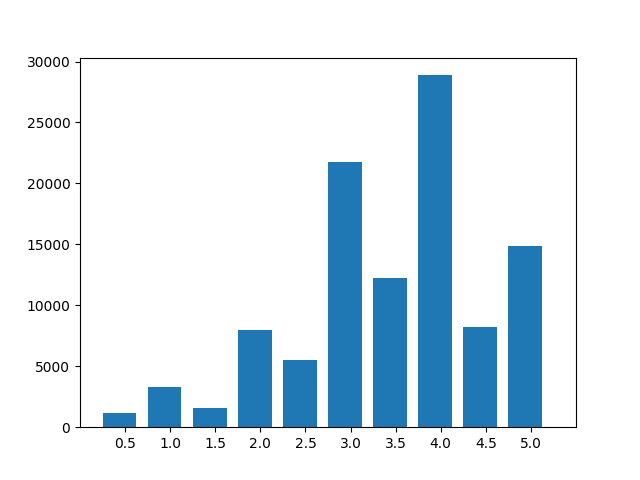
\includegraphics[scale=0.6]{small}
\caption{\emph{small} Movielens dataset ratings distribution}
\end{figure}

\begin{table}[H]
\centering
\begin{tabular}{l|r}
number of users N&  6040 \\ 
number of items M& 3706 \\
average rating & 3.58156 \\
standard deviation & 1.1171 \\
\end{tabular}
\caption{\emph{1M} Movielens dataset statistics}
\end{table}

\begin{figure}[H]
\centering
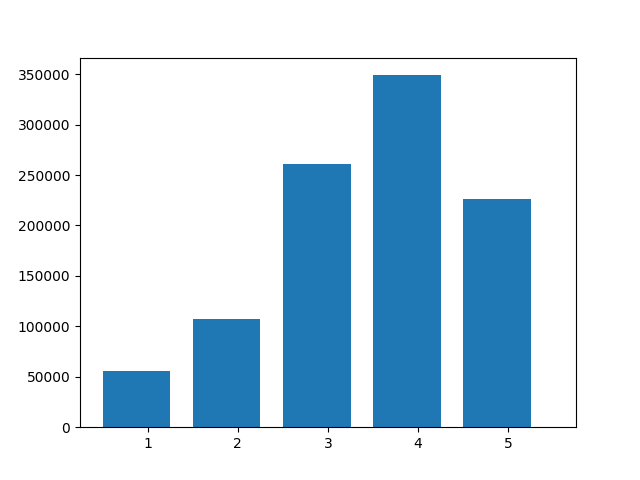
\includegraphics[scale=0.6]{1m}
\caption{\emph{1M} Movielens dataset ratings distribution}
\end{figure}


%\section{VAERec}

VAERec is one of the contributions of this thesis.
It extends the AutoRec model making use of the VAE framework.

It has been implemented in three variants:

\paragraph{U-VAERec} 
reconstructs user rows by learning the conditional distribution
$\ptheta{\ric|\boldui}$ assumed to be a diagonal-covariance Gaussian
and, jointly, the variational approximation to the posterior
$\qphi{\boldui|\ric}$, also assumed to be a diagonal-covariance Gaussian.

\paragraph{I-VAERec} does the same as \emph{U-VAERec}, 
but with item columns, learning $\ptheta{\rcj|\boldvj}$
and $\qphi{\boldvj|\rcj}$.

\paragraph{UI-VAERec} reconstructs a vector consisting of the concatenation
of a user row and item column (FIXME: to be implemented).
It learns $\ptheta{\ric,\rcj|\boldz}$
and $\qphi{\boldz|\ric,\rcj}$.
This differs from the MFVA model with 
the MLP decoder proposed by
\cite{vanBaalen2016}, as a distribution on a 
single latent vector $\boldzij$ representing
the user-item pairing is being produced instead 
of having two distinct distributions on
$\boldui$ and $\boldvj$.

\subsection{Sampling the ratings for the \emph{UI} variants}

Training the \emph{UI-VAERec} would require
have very long epochs, as the number of training
datapoints would be the number of ratings.
To prevent problems related to excessive memory usage,
as one rating would be stored as a concatenation of
its user vector $\ric$ and item vector $\rcj$,
epochs have been implemented as random samplings 
of a fixed amount of the ratings.
The same sampling is performed in the test set.
\subsection{Masking the Adam optimizer}

Given its properties, Adam \cite{KingmaB14} has been choosen
as optimization algorithm.

The VAERec, similarly to the AutoRec, needs to be selective on
which parameters needs to be updated: both in the first
layer of the encoder
and the last layer of the decoder, only the weights
that are connected to existing ratings can be updated.

Provided a binary mask $\mask$ of a parameters tensor $\boldsymbol\theta$
then Adam has the two assignments of $\widehat{\boldm}_t$
and $\widehat{\boldv}_t$ modified from the original algorithm as follows:

\begin{nalign}
\widehat{\boldm}_t &\leftarrow \frac{\boldm_t}{1 - \beta^t_1} \odot \mask
+ \boldm_{t-1}\odot (1-\mask)\\
\widehat{\boldv}_t &\leftarrow \frac{\boldv_t}{1-\beta^t_2}\odot\mask
+ \boldv_{t-1}\odot (1-\mask)
\end{nalign}

%\section{VAERec with Normalizing Flows}

The \emph{VAERec-NF} model
extends the VAERec by improving the posterior approximation
with Normalizing Flows \cite{1505.05770}
as explained in section \ref{iltt}, 
\ref{energy_of_1step_illt}
and \ref{multiple_iltt_steps}.

\subsection{Normalizing Flow using RealNVP's invertible transformation}

In this \emph{VAERec-NF} variant, a transformation of the type previously described
in section \ref{realnvp} is introduced.
This transformation was considered interesting 
because of its implementation
ease and very simple determinant of the Jacobian.
Specifically, the function $s$ is implemented as
a single perceptron layer with nonlinear activation function 
$\tanh$. The function $a$ which is required to be an affine transform,
is implemented as a single perceptron layer with \emph{linear}
activation function.

All the parameters of the transformation are being produced as output of the
encoder network, exactly as happens with the parameters of $\pzcond$ in a Variational
Auto-Encoder.
The weights of the $a$ and $s$ layers are implemented as vectors of size $K^2$, then
reshaped into a $(K,K)$ dimension. This limits the model into
very low latent dimensionalities.

\subsection{Masking}

To ease the implementation, the selection of the first and second parts of $\boldz$
have been implemented with random hyperparameter masks. These masks are unique for each transformation
step, and are computed as follows:

\begin{algorithm}[H]
\caption{Half-full random masks for RealNVP transformations}
\begin{algorithmic}[1]

\REQUIRE ~~\\
(1) Latent dimensionality $K$ \\
(2) Number of transformation steps $k$
\ENSURE~~\\
(1) Random masks $\boldm_1 \ldots \boldm_k$ which have half of their elements set at $1$
`
\item[]
\FOR{$i \in \{1 \ldots k\}$}
\STATE $(\mathbf{a})_j \leftarrow \left\{\begin{array}{ll} 1 & j < K/2 \\ 0 & K/2 \leq i < K\end{array}\right.$
\STATE $\boldm_i = \mathrm{shuffle}(\mathbf{a})$
\ENDFOR
\RETURN $\boldm_1 \ldots \boldm_k$
\end{algorithmic}
\end{algorithm}
                                         
The invertible function, for a transformation step $i$, is hence implemented as:

\begin{nalign}
    \boldz_{i+1} &= \boldz_i\odot\boldm_i + (1-\boldm_i)\odot\left[\boldz_i \odot \exp\left(s(\boldm_i\odot\boldz)\right) + a(\boldm_i\odot\boldz)\right]
\end{nalign}

The masks are computed before training and are left unchanged, as they
should be considered as hyperparameters.

%\section{Dealing with overfitting}

One of the major issues with AutoRec/VaeRec models
is overfitting. The system performs very well on the training
set but unsatisfactory on the test set.

\paragraph{Dropout on the input layer}
Dropout \cite{Srivastava2014}
is a technique aimed at preventing overfitting
which employs randomly dropping units
and their connections
during training.
This would ensure to obtain a neural network
which can function even when parts are deactivated.
Moreover, it would prevent that a single unit becomes
entirely representative of a certain aspect of the training data
data.

It has been observed that applying Dropout on just the input layer
of the VaeRec models,
overfitting can be prevented to a certain degree,
possibly by a similar way of action as denoising autoencoders.
\cite{Vincent2010}.

\paragraph{Narrowing the bottleneck}
\paragraph{Regularization}
Regularization has been tested with either L1 or L2 norms,
without significant improvements.
\paragraph{Batch Normalization}
\paragraph{Increasing the depth}
FIXME:explain paper \cite{MhaskarLP17}

%\section{Representation Learning}
Representation Learning (RL) is a developing branch of Machine Learning that has one of its
focuses on extracting representations codes $$\mathbf{Z} = \{\mathbf{z}_i\}_{i=1}^N$$ from the datapoints in a dataset $$\mathbf{X} = \{\mathrm{x}_i\}_{i=1}^N$$.
It is usually desirable for these representations to be characterized by properties such as low-dimensionality, clusterability, increased linear separability (especially when used for further classification tasks) and intuitive "semantic" explainability of the dimensions of the learned manifold.

One common attempt to achieve such properties is the use of Principal Component Analysis (PCA) , which transforms the original features of the raw input into a set of uncorrelated variables.
The main drawback of PCA is the assumption that the explaining dimensions are linearly related to the directions of maximum variance in the data.
This assumption is not true for most complex datasets, in which the original features of a dataset might actually be the result of arbitrarly complicated nonlinear unknown functions.

For this reason alternative approaches to RL are being employed, such as Autoencoders (AE) as specific forms of Artificial Neural Networks (ANN).
AEs have typically a "diabolo" shape, as an arbitrarly highly dimensional input is progressively being reduced to lower dimensionalities over layers of progressively shrinking sizes.
This part of the neural network is an encoder, as its purpose is to generate low-dimensional compressed codes from a high-dimensional input.
The last layer of the encoder is the smallest layer of the network, hence called bottleneck.
To the bottleneck is attached a decoder network with layers of progressively increasing size.
The last layer of the decoder is matching the dimensionality of the input layer.
The learning of the network's parameters is performed by minimizing an objective function containing the error between the reconstruction output of the network and its input.
This objective function is then minimized via Gradient Descent and its variants.

%\section{Scaling issues and regularization}

In order to achieve the same intensity of learning per epoch even by varying
the minibatch size it is necessary to re-scale some hyperparameters.

Let's consider a complete objective for a typical learning task
of quantities $y_i$ from respective datapoints $x_i$, using
a dataset $\mathcal{D} = \{x_i,y_i\}_i^{|D|}$.
As the datapoints
are independent and identically-distributed, then it can be expressed as a sum over
all the datapoints.
One step of learning from this objective is usually referred as an "epoch".

\begin{nalign}
\label{complete_J}
J = \sum_{i=1}^{|\mathcal{D}|}
\ell(x_i,y_i) + \lambda \Omega(\Theta)
\end{nalign}

Where $\Omega$ is a regularization term, $\Theta$ is the set of the regularizable
parameters and $\lambda$ is a fixed hyperparamter that determines the regularization amount.

This objective is subject to Gradient Descent learning on the trainable parameters:

\begin{nalign}
\Theta_{t+1} = \Theta_t - \gamma\nabla_\Theta J_t
\end{nalign}

Where $\gamma$ is the learning rate hyperparameter.

As $J$ is defined as a sum over independent datapoints, it is possible to use Stochastic
Gradient Descent learning strategies, which take into account only a limited number of datapoints at each time.

It's desirable to consider the average contribution of each datapoint to the objective
$J$ \ref{complete_J}:

\begin{nalign}
\label{average_datapoint_J}
J_a = 
\frac{1}{|\mathcal{D}|}
J =
\frac{1}{|\mathcal{D}|}
\sum_{i=1}^{|\mathcal{D}|}
\ell(x_i,y_i) + \frac{\lambda}{|\mathcal{D}|} \Omega(\Theta)
\end{nalign}

If learning using $J_a$ is repeated $|\mathcal{D}|$ times within an epoch, then
the algorithm achieves the same learning intensity as
with $J$ by keeping the same learning rate $\gamma$.

By considering splitting the dataset and the objective $J$ 
\ref{complete_J} into a number of minibatches of size $B$, an approximation to $J_a$,
useful for SGD-like algorithms,
can be obtained:

\begin{nalign}
J_b = \frac{1}{B}\sum_{i=1}^{B} \ell (x_i, y_i) + \frac{\lambda}{|\mathcal{D}|}\Omega(\Theta)
\end{nalign}

An important consequence of using $J_b$ is that the intensity of the learning 
is altered,
because less updates would be applied to $\Theta$ at each epoch.
In order to balance this phenomenon, the learning rule can be modified as follows:

\begin{nalign}
\Theta_{t+1} = \Theta_t - B\gamma\nabla_\Theta J_{b,t}
\end{nalign}



%\section{RPROP update algorithm}

\emph{RPROP}\cite{rprop} is a gradient-based parameter update schema that does not take into account the magnitudes of the gradients, but only their sign.

The idea is simple: if the gradient keep pointing towards the same (either positive or negative) direction,
then the parameter-specific update delta needs to be increased, otherwise, in case
the gradient for a parameter keeps changing sign, then the update delta needs to decrease,
in order to fine-tune the parameter to its optimum.

The change of variation is detected by the product of the gradient of an parameter $w_i$
calculated to minimize an objective function $J$
parameter a time step $t$ by the gradient of that same parameter at the previous time step $t-1$:

\begin{nalign}
p &= \left(\frac{\partial J}{\partial w_i}\right)^{(t-1)}
* \left(\frac{\partial J}{\partial w_i}\right)^{(t)}
\end{nalign}
       
The sign of $p$ determines the increase or decrease of the parameter-specific delta $\Delta_i$:
\begin{nalign}
\Delta_i^{(t)} =
\left\{
\begin{array}{lll}
 \min \{ \eta^+ * \Delta_i^{(t-1)} , \Delta_{\mathrm{max}} \} & \mathrm{if} & p > 0\\
 \max \{ \eta^- * \Delta_i^{(t-1)} , \Delta_{\mathrm{min}} \} & \mathrm{if} & p < 0\\
 \Delta_i^{(t-1)} & \mathrm{if} & p = 0
\end{array}
\right. 
\end{nalign}

Where $ 0 < \eta^- < 1 < \eta^+ $.

Typical parameter settings are $\eta^- = 0.5$, $\eta^+ = 1.2$, $\Delta_{\mathrm{min}} = 1e^{-6}$,
$\Delta_{\mathrm{max}} = 50.0$ and initial delta values $\Delta_0 = 0.1$.


%\section{Technologies used}

\paragraph{Python version 3}
The Python programming language is well suited for data science applications. Its large
number of libraries available makes it suitable for avoiding re-inventing the wheel.
Its conciseness make it very readable and hands-on.

\paragraph{Theano} \cite{theano}
It's a Python library useful to create computational graphs and automatic differentiation,
specifically using tensors.

\paragraph{DAS4} \cite{das}
Grid computing environment from a partnership between Dutch universities. Allows the use
of concurrent jobs, also on nodes that are provided with GPUs to speed-up deep learning
computations.


\bibliography{references.bib}
\bibliographystyle{apalike}
\end{document}
